%%% Local Variables:
%%% mode: latex
%%% TeX-master: t
%%% End:

\documentclass[master,nofonts]{thuthesis}
%\documentclass[master]{thuthesis}
%\documentclass[doctor]{thuthesis}
% \documentclass[%
%   bachelor|master|doctor|postdoctor, % mandatory option
%   winfonts|nofonts|adobefonts, % mandatory only for bachelor and Linuxer
%   secret,
%   openany|openright,
%   arialtoc,arialtitle]{thuthesis}
% 当使用 XeLaTeX 编译时,本科生、Linux 用户需要加上 nofonts 选项;
% 当使用 PDFLaTeX 编译时,adobefonts 选项等效于 winfonts 选项(缺省选项)。

% 所有其它可能用到的包都统一放到这里了,可以根据自己的实际添加或者删除。
\usepackage{thutils}
\usepackage{cases}
\usepackage{tabularx}
\usepackage{epstopdf}
\usepackage{footmisc}
\usepackage{pdfpages}
\usepackage{bm}
\usepackage{lscape}
\usepackage{tikz}
\usepackage{tikzscale}
\usepackage[justification=centering]{subcaption}

%\usepackage{pgfplots} 

\usepackage{algorithm} %%format of the algorithm
\usepackage{algorithmicx} %%format of the algorithm
\usepackage{algpseudocode}
\floatname{algorithm}{算法}
\renewcommand{\algorithmicrequire}{\textbf{输入:}} %%Use Input in the format of Algorithm
\renewcommand{\algorithmicensure}{\textbf{输出:}} %%UseOutput in the format of Algorithm
%\algrenewcommand{\algorithmiccomment}[1]{\hskip3em $\rightarrow$ #1}
\algrenewcommand{\algorithmiccomment}[1]{ $//$ #1}
 
\usepackage{listings}
\renewcommand\lstlistingname{代码}
\renewcommand\lstlistlistingname{代码}

\lstset{framexleftmargin=1.4em, basicstyle=\ttfamily\small,
        %frame=shadowbox, numberstyle=\tiny, breaklines=true,
        frame=single,
        numberstyle=\tiny, breaklines=true,
        keywordstyle=\color{blue!70}\bfseries,
        %commentstyle=\color{red!50!green!50!blue!50},
        rulesepcolor=\color{red!20!green!20!blue!20},
        xleftmargin=1.8em, numbers=none,fontadjust=true}
\lstdefinelanguage{shader}{morekeywords={uniform, layout, uniform, vec2, vec3, vec4, in, out, gl_Position, dot, flat, int ,float, gl_VertexID, xyz, w, x, y, z, location, version, sampler2DRect, bgr, gl_FragData, texture2DRect, gl_TexCoord},morecomment=[l]{//}}

\usepackage{placeins}
\makeatletter
\AtBeginDocument{%
  \expandafter\renewcommand\expandafter\subsection\expandafter
    {\expandafter\@fb@secFB\subsection}%
  \newcommand\@fb@secFB{\FloatBarrier
    \gdef\@fb@afterHHook{\@fb@topbarrier \gdef\@fb@afterHHook{}}}%
  \g@addto@macro\@afterheading{\@fb@afterHHook}%
  \gdef\@fb@afterHHook{}%
}
\makeatother

\def\fourgraphicswidth{0.45} %0.3\textwidth

% 你可以在这里修改配置文件中的定义,导言区可以使用中文。
\def\myname{唐磊}

\begin{document}

%\selectcolormodel{gray} 

% 定义所有的eps文件在 figures 子目录下
\graphicspath{{figures/}}


%%% 封面部分
\frontmatter

%%% Local Variables:
%%% mode: latex
%%% TeX-master: t
%%% End:
\secretlevel{绝密} \secretyear{2100}

\ctitle{凸包围多面体生成算法及应用}
% 根据自己的情况选,不用这样复杂
\makeatletter
\ifthu@bachelor\relax\else
  \ifthu@doctor
    \cdegree{工学博士}
  \else
    \ifthu@master
      \cdegree{工学硕士}
    \fi
  \fi
\fi
\makeatother


\cdepartment[软件学院]{软件学院}
\cmajor{软件工程}
\cauthor{唐磊} 
\csupervisor{雍俊海教授}
% 如果没有副指导老师或者联合指导老师,把下面两行相应的删除即可。
% \cassosupervisor{陈文光教授}
% \ccosupervisor{某某某教授}
% 日期自动生成,如果你要自己写就改这个cdate
%\cdate{\CJKdigits{\the\year}年\CJKnumber{\the\month}月}

% 博士后部分
% \cfirstdiscipline{计算机科学与技术}
% \cseconddiscipline{系统结构}
% \postdoctordate{2009年7月——2011年7月}

\etitle{Convex Bounding Polyhedron Construction and its Application} 
% 这块比较复杂,需要分情况讨论:
% 1. 学术型硕士
%    \edegree:必须为Master of Arts或Master of Science(注意大小写)
%              “哲学、文学、历史学、法学、教育学、艺术学门类,公共管理学科
%               填写Master of Arts,其它填写Master of Science”
%    \emajor:“获得一级学科授权的学科填写一级学科名称,其它填写二级学科名称”
% 2. 专业型硕士
%    \edegree:“填写专业学位英文名称全称”
%    \emajor:“工程硕士填写工程领域,其它专业学位不填写此项”
% 3. 学术型博士
%    \edegree:Doctor of Philosophy(注意大小写)
%    \emajor:“获得一级学科授权的学科填写一级学科名称,其它填写二级学科名称”
% 4. 专业型博士
%    \edegree:“填写专业学位英文名称全称”
%    \emajor:不填写此项
\edegree{Master of Science} 
\emajor{Software Engineering} 
\eauthor{Tang Lei} 
\esupervisor{Professor Yong Junhai} 
% \eassosupervisor{Chen Wenguang} 
% 这个日期也会自动生成,你要改么?
% \edate{December, 2005}

% 定义中英文摘要和关键字
\begin{cabstract}
  
在计算机辅助设计、计算机动画和计算机图形学等领域中,包围盒的应用十分广泛,根据其相交测试的简单性常用于对其包围原始模型之间的如几何求交、光线跟踪或者碰撞
检测等多种算法进行预判,以提高整体算法的效率。
凸包围多面体作为包围盒的推广,对于一般不规则形体,可达到比包围盒更好的紧致程度,因而能够更好地对相关算法进行预判剪枝以提高效率。

本文提出了一种快速构造给定点集的指定~$k$~面的紧致凸包围多面体($k$ - Convex Bounding Polyhedron, 简称~$k$-CBP)的方法。
该方法首先利用一个线性算法对输入点集构造一个近似内凸包, 然后根据该内凸包的面片法向通过~$k$-means~聚类算法生成构造凸包围多面体的~$k$~个截面法向,
然后扫描输入点集依次沿各个法向搜索切点构造构成凸包围多面体的截面,最后通过截面求交构成~$k$-CBP。 
在搜索截面的过程中,各个法向之间的搜索过程相互独立,可以方便地进行并行搜索,本文分别基于~OpenGL~着手语言和~CUDA~两种平台提供了并行加速的方案。
在截面求交过程中,本文利用计算几何中的对偶映射技术加快求交过程。
实验结果表明,与同类算法相比,本文方法能够更快地构造给定点集更加紧致的凸包围多面体。

碰撞检测算法一直是计算机动画和计算机图形学领域中研究热点,本文在常用的层次结构包围盒树方法的基础上,
利用构造模型的~$k$-CBP~进行预判剪枝,提出了一种基于~$k$-CBP~的碰撞检测算法。
该方法首先构造模型的包围盒,通过包围盒相交检测的模型须通过~$k$-CBP~的相交检测才能进行真实模型的相交检测。
本文在~$k$-CBP~之间的相交测试过程中,利用了一种基于包围盒树的方法和一种计算基于凸体模型之间的距离的方法进行相交测试,
实验结果表明该在静态或运动场景的碰撞检测环境中均达到良好的剪枝效果,有助于提高碰撞检测算法的效率。


%  本文的创新点主要有:
%  \begin{itemize}
%    \item 用例子来解释模板的使用方法;
%    \item 用废话来填充无关紧要的部分;
%    \item 一边学习摸索一边编写新代码。
%  \end{itemize}

\end{cabstract}

\ckeywords{凸包围体, 近似凸包, 并行计算, 碰撞检测}

\begin{eabstract} 
   [TODO] An abstract of a dissertation is a summary and extraction of research work
   and contributions. Included in an abstract should be description of research
   topic and research objective, brief introduction to methodology and research
   process, and summarization of conclusion and contributions of the
   research. An abstract should be characterized by independence and clarity and
   carry identical information with the dissertation. It should be such that the
   general idea and major contributions of the dissertation are conveyed without
   reading the dissertation. 

   An abstract should be concise and to the point. It is a misunderstanding to
   make an abstract an outline of the dissertation and words ``the first
   chapter'', ``the second chapter'' and the like should be avoided in the
   abstract.

   Key words are terms used in a dissertation for indexing, reflecting core
   information of the dissertation. An abstract may contain a maximum of 5 key
   words, with semi-colons used in between to separate one another.
\end{eabstract}

\ekeywords{Convex bounding volume, Approximate Convex hull, Parallel computing,
Collision detection}

% 设置 PDF 文档的作者、主题等属性
\makeatletter
\thu@setup@pdfinfo
\makeatother
\makecover

% 目录
\tableofcontents

% 符号对照表
\begin{denotation}

\item[BV] 包围体~(Bounding Volume)
\item[CH] 凸包~(Convex Hull)
\item[$\tau$] 包围体的紧致性 
\item[$\Delta G$]  	活化自由能~(Activation Free Energy)
\item [$\chi$] 传输系数~(Transmission Coefficient)
\item[$E$] 能量
\item[$m$] 质量
\item[$c$] 光速
\item[$P$] 概率
\item[$T$] 时间
\item[$v$] 速度
\item[劝  学] 君子曰:学不可以已。青,取之于蓝,而青于蓝;冰,水为之,而寒于水。
  木直中绳。(车柔)以为轮,其曲中规。虽有槁暴,不复挺者,(车柔)使之然也。故木
  受绳则直, 金就砺则利,君子博学而日参省乎己,则知明而行无过矣。吾尝终日而思
  矣,  不如须臾之所学也;吾尝(足齐)而望矣,不如登高之博见也。登高而招,臂非加
  长也,  而见者远;  顺风而呼,  声非加疾也,而闻者彰。假舆马者,非利足也,而致
  千里;假舟楫者,非能水也,而绝江河,  君子生非异也,善假于物也。积土成山,风雨
  兴焉;积水成渊,蛟龙生焉;积善成德,而神明自得,圣心备焉。故不积跬步,无以至千
  里;不积小流,无以成江海。骐骥一跃,不能十步;驽马十驾,功在不舍。锲而舍之,朽
  木不折;  锲而不舍,金石可镂。蚓无爪牙之利,筋骨之强,上食埃土,下饮黄泉,用心
  一也。蟹六跪而二螯,非蛇鳝之穴无可寄托者,用心躁也。\pozhehao{} 荀况
\end{denotation}



%%% 正文部分
\mainmatter

%%% Local Variables:
%%% mode: latex
%%% TeX-master: t
%%% End:

\chapter{引言}
\label{cha:intro}

本章将介绍本文的相关背景,常用的凸包围体种类及应用,常见的碰撞检测算法及本文的结构安排。


TODO 图表用中文表示


\section{相关背景}

随着计算机软硬件技术的不断升级和发展,人们的衣食住行都越来越离不开计算机。
计算机图形学、计算机动画和虚拟现实等相关技术已经融入人类的日常生活当中,成为人们生活的重要组成部分,如医学领域的虚拟手术、设计领域的三维建模造型技术,日常生活中的电影游戏等等。

凸包围体技术在计算机图形学领域里的各种算法中发挥着重要作用,
如优化渲染和建模,加速求交、碰撞检测等。
以求交算法为例,如果两个模型相交,则对应的凸包围体一定相交,若凸包围体不相交则原始模型一定不相交。
凸包围体作为原始模型的近似,通常情况下,判断凸包围体是否相交比判断原始模型相交更简单,因此利用这个性质就可以加速模型之间的相交检测。
计算机图形学领域里常见的~AABB(Axis Aligned Bounding Box)包围盒和计算几何领域里的凸包都是凸包围体。
凸包围体有多种应用,主要是利用其“凸”的性质和可用来近似被包含模型的特征,应用于模型化简、碰撞检测等。
在几何计算过程中,包围体也用于相交等操作中进行预判和剪枝以提升整体算法的运行效率。

碰撞检测问题是计算机图形学、虚拟现实等领域中的研究热点,是计算机模拟真实环境中不可或缺的技术,在物理仿真及游戏领域里应用广泛。
例如在游戏中,碰撞检测技术增强了游戏的真实性,游戏中的角色行走不可穿墙、角色中弹而亡等等都离不开碰撞检测技术。

下面将分别介绍凸包围体相关技术和碰撞检测相关算法。

\section{凸包围体}
\label{sec:convex-bv}

对于“凸”定义如下(以二维欧式空间为例):
给定点集$S = \{p_1, ..., p_n\} \subseteq E^2$,如果有
$\lambda = (\lambda_1,...,\lambda_n)^T \in R^n, \lambda_1 + ... + \lambda_n = 1
$~且~ $min\{\lambda_1,...\lambda_n\} \geq 0$,我们称点 $p = [p_1, ... ,
p_n]\lambda = \lambda_1 p_1 + ... + \lambda_n
p_n$~为~$S$~的一个凸组合。一个点集~$P \subseteq E^2$~为凸的集合,当且尽当~$P$~的子集的凸组合仍然是$P$的子集。
更形象地讲,如果一个二维欧式空间的多边形是凸的,那么连接任意多边形内的两点构成的线段仍然在这个多边形的内部。

凸包围体能用于在原始模型之间的相关计算(遮挡测试、相交测试等)之前进行预处理判断和裁剪的理论基础正是基于此。通常来讲(无特别强调,本文不考虑包围体比原始模型还复杂的情况),凸包围体之间的计算比包含的原始模型计算更简单,当凸包围体之间没有相交或遮挡时,原始模型一定没有相交或遮挡。

根据具体的应用场景的不同有不同形状的凸包围体,常见的如下。

\subsection{AABB 包围体}

AABB(Asix Aligned Bounding Box)包围体是最常见最简单的包围体,俗称包围盒,其方向始终沿着坐标轴方向\cite{bergen1997efficient}。
在平面中就是包含二维模型的矩形,如图\ref{fig:aabb-bunny}所示,为平面图形~Bunny~的~AABB~包围体(二维情况称包围矩形更合适,但为了统一,这里统称包围体,后同)。对应到三维空间中就是沿坐标轴方向包含模型的最小的长方体。

\begin{figure}[H] % use float package if you want it here
  \centering
  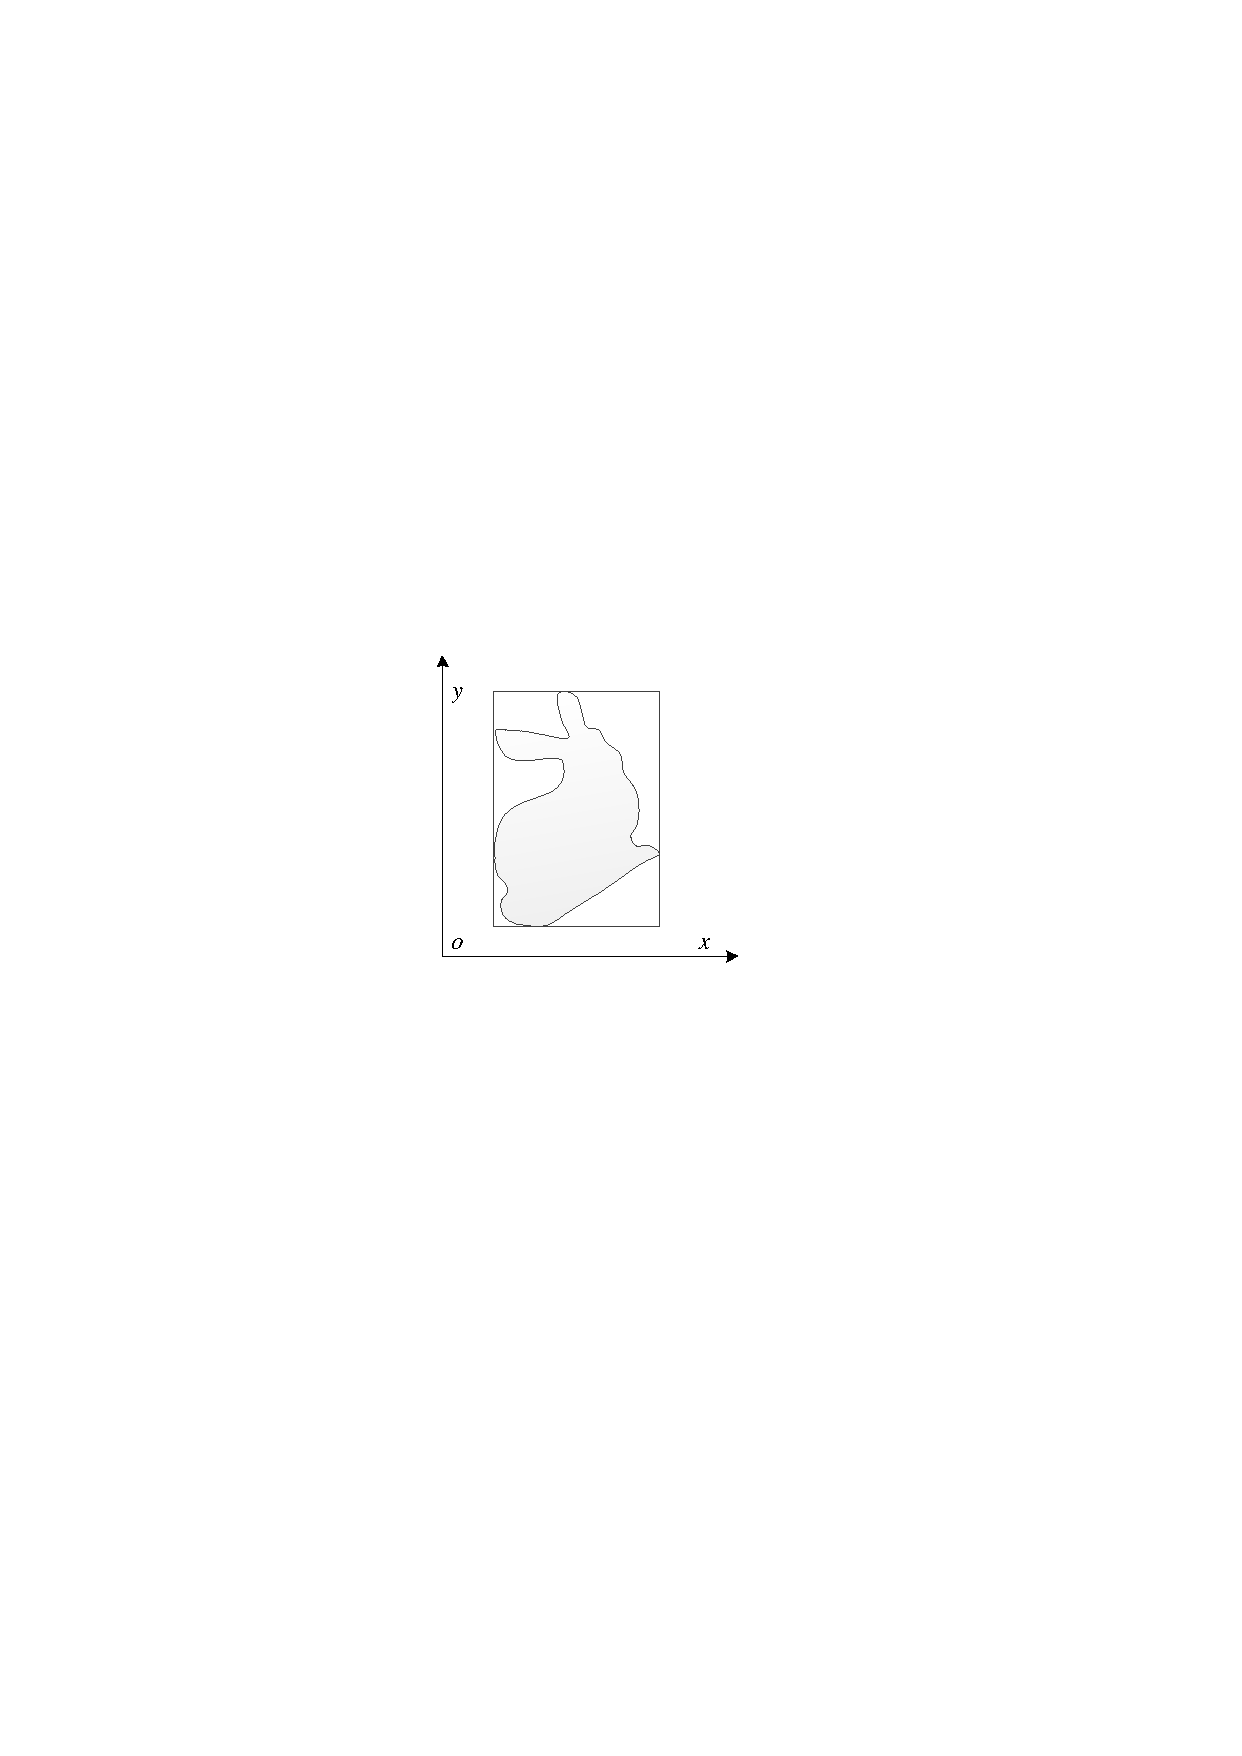
\includegraphics[width=1.5in]{bunny-2d-AABB.pdf}
  \caption{AABB 包围体}
  \label{fig:aabb-bunny}
\end{figure}

AABB~包围体的数据结构通常有3种方式:
\begin{inparaenum}[(1)]
\item 存储~AABB~包围体对角线上的两个极点,$Point_{min}$和$Point_{max}$,著名的计算几何库~CGAL\footnote{CGAL, Computational Geometry Algorithms Library, http://www.cgal.org}以此种方式存储;
\item 存储~AABB~包围体的中心点和各个方向的半径,$Point_{center}$和$Vector_{radius}$,如~SOLID\cite{bergen1997efficient};
\item 存储~AABB~包围体的极小点和各个方向的延伸长度\cite{ericson2005real},$Point_{min}$和$Vector_{extent}$。
\end{inparaenum} 

一方面~AABB~包围体之间的相交测试较简单,以数据结构为存储两个极点为例,只需要比较各个坐标值之间的大小即可。
但另一方面,通常情况下与原始模型的近似性较差,因其包围体的边沿着坐标轴方向可能会留较多的空白空间。

\subsection{OBB 包围体}

~OBB(Oriented Bounding Box)包围体是带方向的包围盒,可看作是~AABB~包围体沿任意方向转动一定角度后构成的包围体,因此通常情况下,~OBB~较~AABB~而言可以更紧致地贴近原始模型。
如图\ref{fig:obb-bunny}所示为平面图形~Bunny~的~OBB~包围体。

\begin{figure}[H] % use float package if you want it here
  \centering
  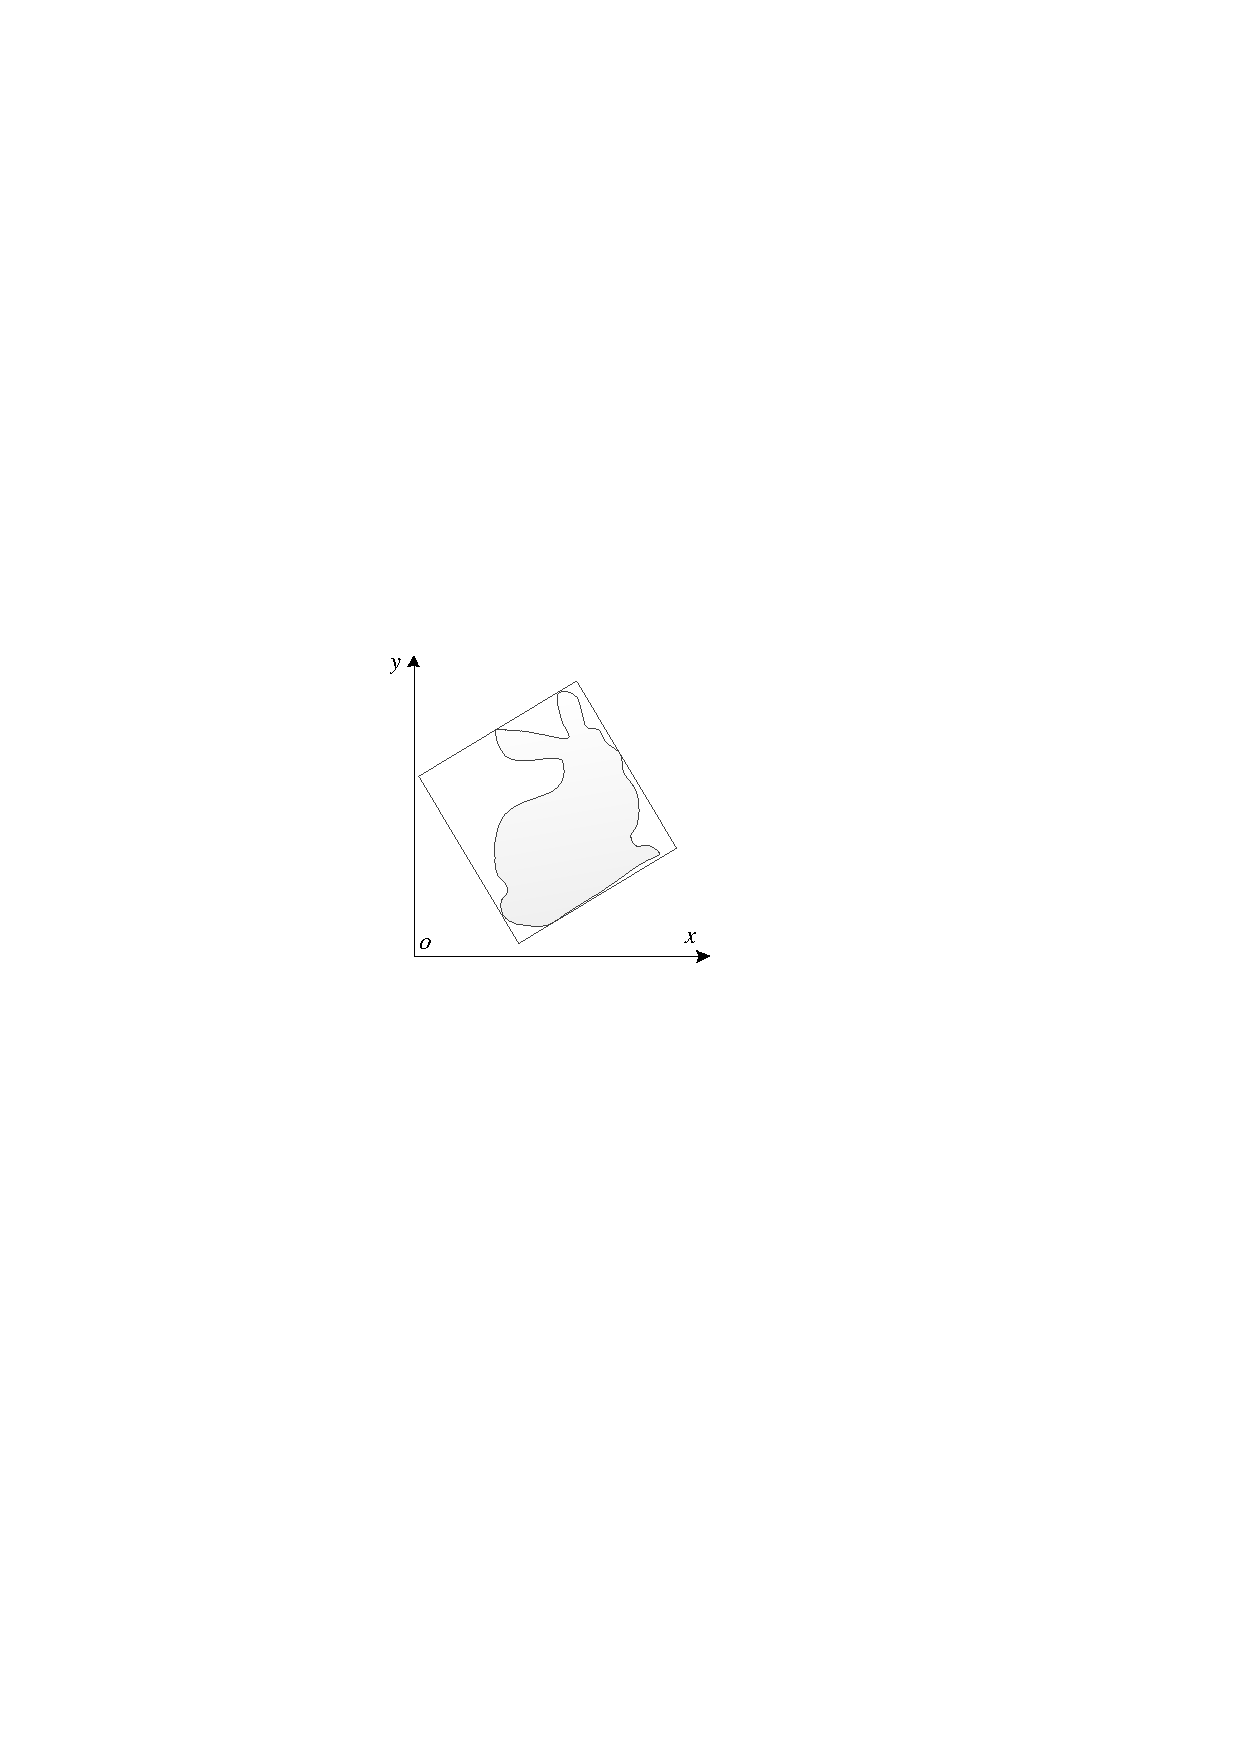
\includegraphics[width=1.5in]{bunny-2d-OBB.pdf}
  \caption{OBB 包围体}
  \label{fig:obb-bunny}
\end{figure}

与~AABB~类似,OBB~包围体的数据存储方式也可以有多种,最常用的是存储中心点,局部坐标架以及各个方向上的半径\cite{gottschalk1996obbtree}。因为~OBB~包围体的方向是任意的,有不少学者研究如何得到更加紧致的~OBB。

最早可追溯到由~O'Rourke~\cite{o1985finding}提出的$O(n^3)$
算法,文献\onlinecite{barequet2001efficiently}中提出了一种方法理论上可以在$O(n
+ 1/ \epsilon ^{4.5} )$复杂度内计算出一个近似最小~OBB($\epsilon$
为近似误差,即得到的$V\leq(1+\epsilon)\times V_{min}$,
其中$V$表示~OBB~的体积,$V_{min}$为最小~OBB~的体积),实际应用中通常实现的算法复杂度为$O(nlogn + n/
\epsilon ^{3} )$。~C.K.Chan~ \cite{chan2001determination}
提出了另外一种迭代的算法可以计算出误差范围内最小的~OBB~包围体,该算法适用于点数量较多(超过1万个点)的模型。

与~AABB~相比,~OBB~之间的相交测试稍复杂,需将二者转换到同一坐标系下进行计算,但其能更好的逼近原始模型。

\subsection{Sphere 包围体}

球形(Sphere)包围体,也称包围球(二维情况下即为包围圆,下同),即用一个半径尽量小的球包住给定所有点,该问题的求解是计算几何中的经典问题最小包围球的变种。
如图\ref{fig:sphere-bunny}所示为平面图形~Bunny~的~Sphere~包围体。

\begin{figure}[H] % use float package if you want it here
  \centering
  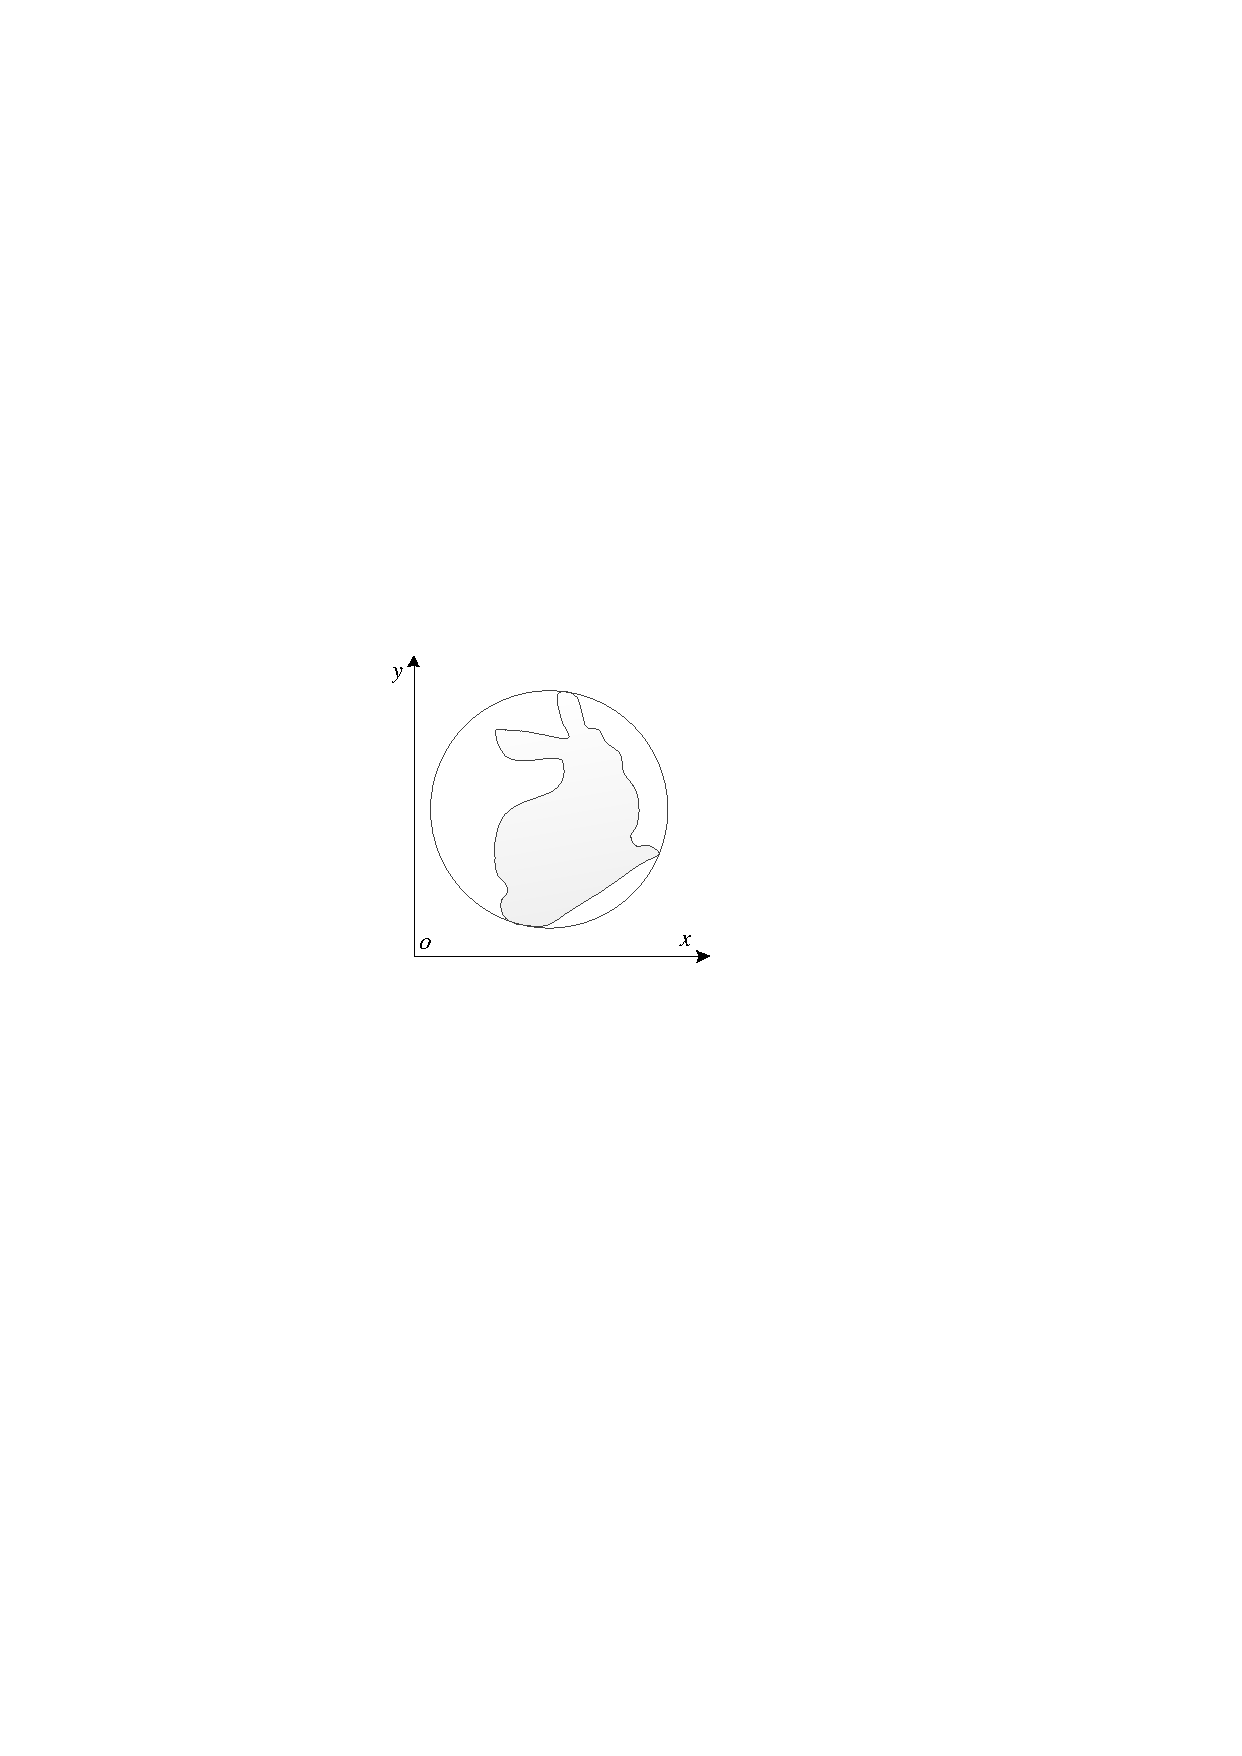
\includegraphics[width=1.5in]{bunny-2d-Sphere.pdf}
  \caption{Sphere 包围体}
  \label{fig:sphere-bunny}
\end{figure}

包围球的数据结构较简单,只需要球心和半径。一种最简单的计算一个包围求的方法是将相应~AABB~包围体的中心点作为球心,半径是为~AABB~各方向半径的最大值,这种方法虽然计算较快,但得到的包围体往往不够紧致。为了得到最小包围球,~E.Welzl~\cite{Welzl1991Smallest}
提出了一种线性的随机算法求出最小包围球。~T.Larsson~\cite{larsson2008fast}提出了一种快速简单的算法,该算法基于选择$k$个极点生成$k/2$个方向构造包围球,因而称为~EPOS~(Extremal Points Optimal Sphere~)算法,可以自定义$k$ 的值,能够给执行时间和包围盒紧致性之间进行调整折衷,提高了灵活性。

测试两个包围球是否相交较简单,只需判断两个球心之间的距离是否大于两个球半径之和即可。

\subsection{$k$-DOP 包围体}

$k$-DOP(Discrete Orientation Polytope)包围体是一个由$k$个固定方向的半平面相交构成的凸多面体,其最早思想来源于~TL.Kay~\cite{Kay1986Ray}
等人提出的用于解决光线追踪的问题,~$k$-DOP~术语是由~J.Klosowski~等人\cite{klosowski1998efficient}
在1998 年用于解决碰撞检测问题时提出的,有学者也称~$k$-DOP~为$k$-FDH($k$-Fixed
Directions Hull)\cite{weiyingmei2001}。
在二维(三维)平面上,~k-DOP~就是一个由$k/2$对平行的固定方向的边(面)围成的凸多边形(多面体),其中$k\in\mathbb{N}$,$k\geq4$($k\geq6$)。如图\ref{fig:8dop-bunny}所示,为平面图形~Bunny~的$8$-DOP。

\begin{figure}[H] % use float package if you want it here
  \centering
  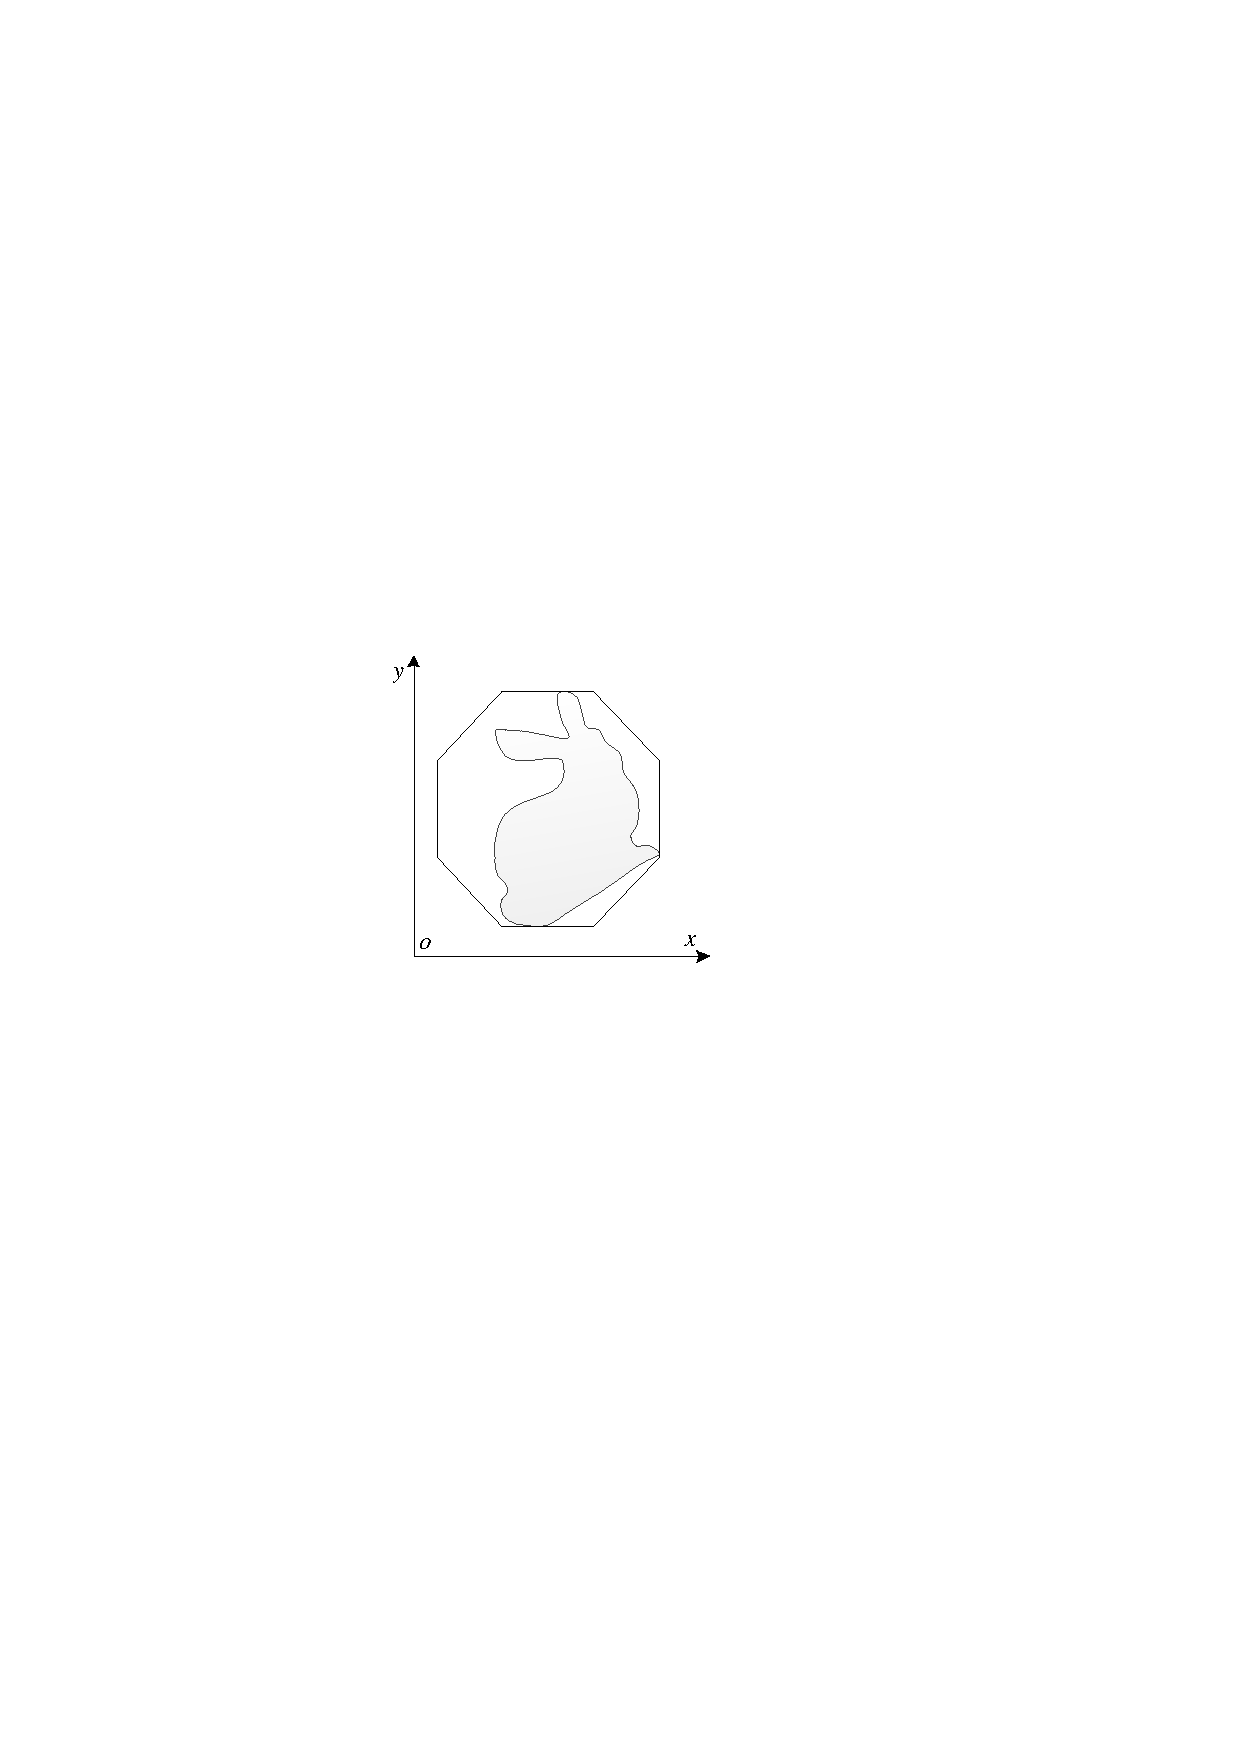
\includegraphics[width=1.5in]{bunny-2d-8DOP.pdf}
  \caption{$k$-DOP 包围体($k=8$)}
  \label{fig:8dop-bunny}
\end{figure}

对于$k$-DOP~中的每一个方向,可以由相应边(面)的法向决定,其数据结构一般用$k/2$个半平面的法向,再加上模型在各个方向上的投影的极值即可。因为$k$-DOP~的方向固定,$k$值确定后,相应的法向也随即确定,所以只需要存储各个方向的极值即可。当$k$-DOP~用于碰撞检测或可视化时,一般还需存储包围体的各个顶点。

与其他几种包围盒相比较而言,$k$-DOP~是取包围体存储计算和相交测试耗费时间的一个折衷,且可以通过修改$k$的值来提高包围体的灵活性。

\subsection{Convex hull 包围体}

凸包(Convex hull)是在计算几何中出现的概念,被定义为包含点集模型的最小凸集\cite{dengcg},
因此~Convex hull~包围体是最紧致的凸包围体,能够更好地近似模型本身。
包围体的紧致程度以凸包为衡量标准,一个包围体的紧致性 $\tau$ 按照如下公式计算:

\begin{equation}
\tau = \frac{V(CH)}{V(BV)}
\end{equation}
其中,$V(CH)$为凸包的体积,$V(BV)$~为包围体的体积,按照此公式计算出来的$\tau$越接近1表明其越紧致,凸包最紧致,其紧致性值1。

图\ref{fig:convexhull-bunny}为二维凸包的示例。

\begin{figure}[H] % use float package if you want it here
  \centering
  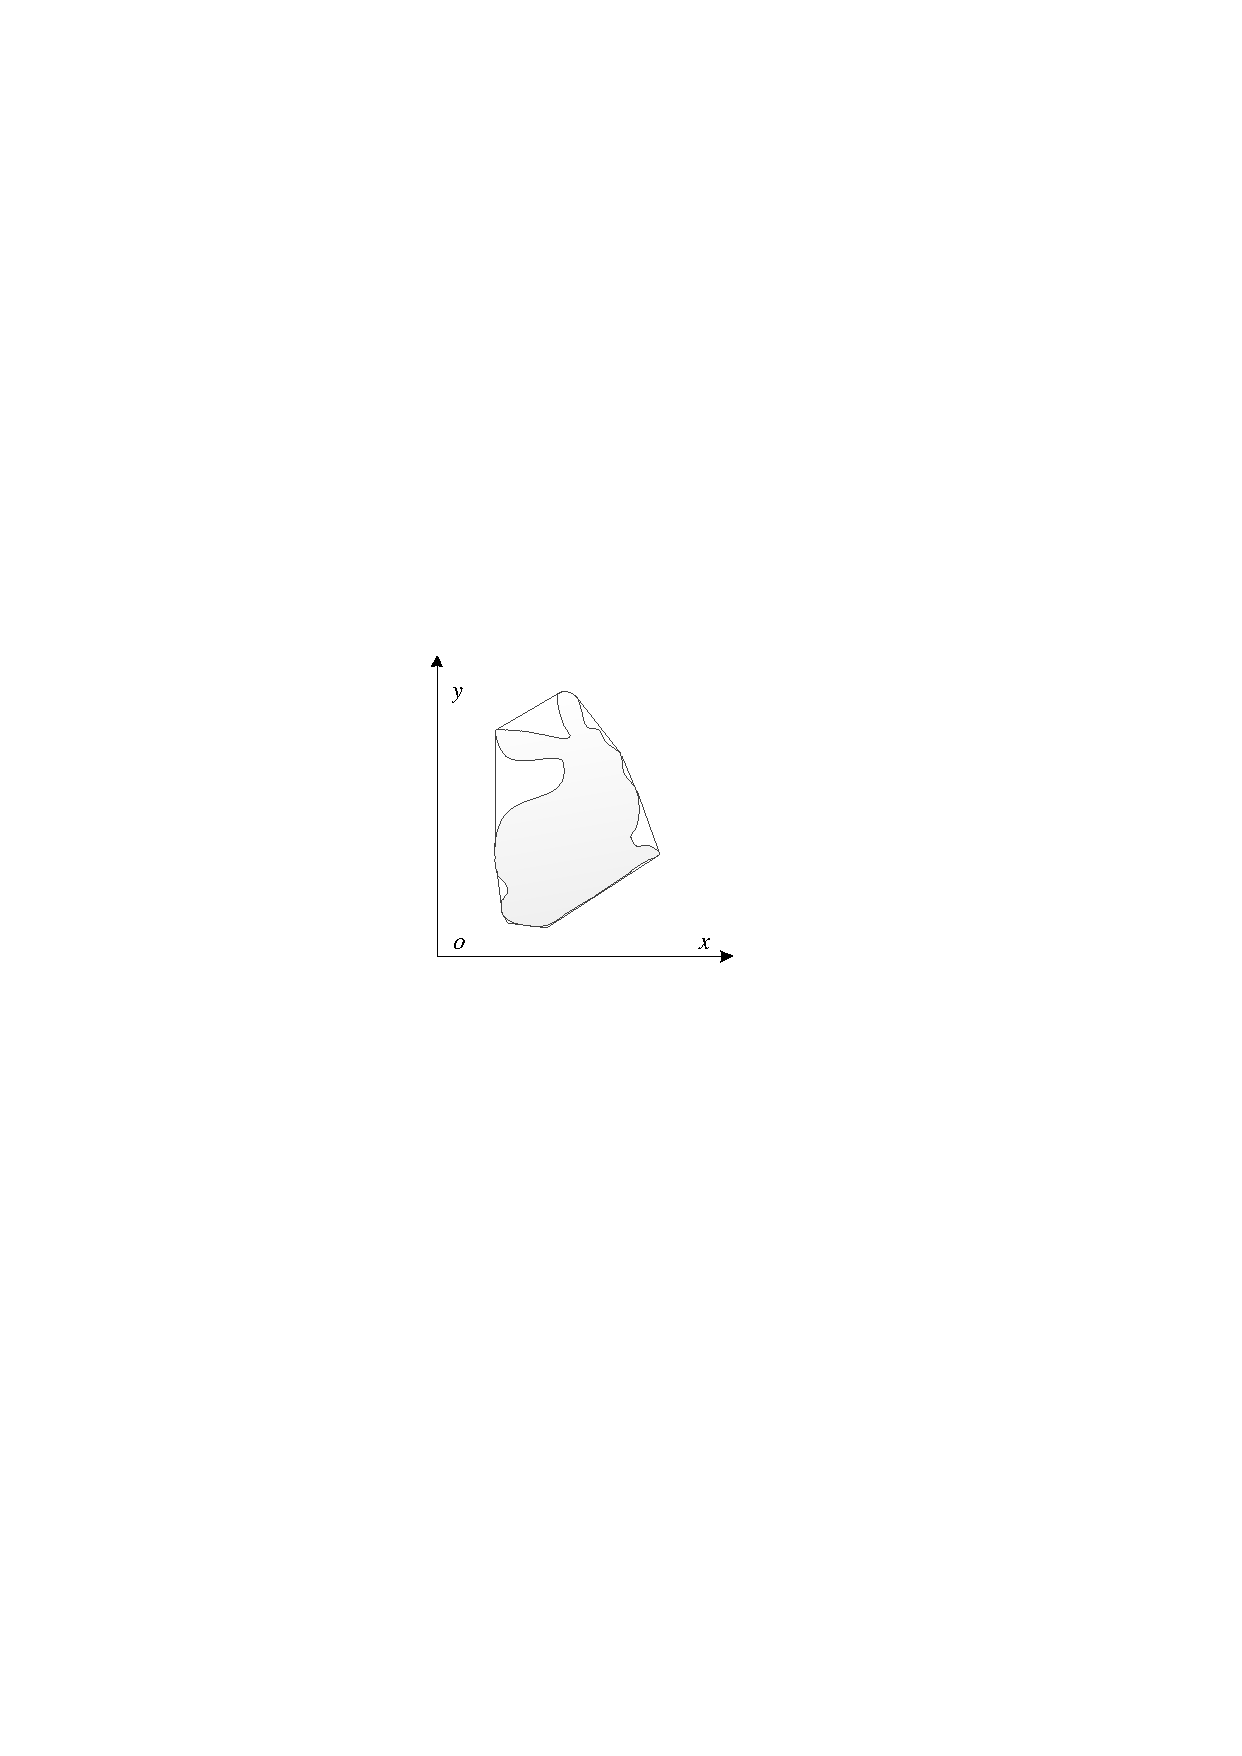
\includegraphics[width=1.5in]{bunny-2d-Convexhull.pdf}
  \caption{Convex hull 包围体}
  \label{fig:convexhull-bunny}
\end{figure}

常用的凸包构造算法有~Gift wrapping~\cite{Chand1970An},复杂度最坏情况下为$O(n^2)$,构造凸包的算法时间复杂度下限为$O(n\log n)$,如~Preparata~提出的分治算法\cite{Preparata1977}。
当模型点集较大时,包围体涉及到的面片数量太多,做相交测试等相关计算时耗费时间较久,同时也耗费较多存储空间。因此~Convex hull~包围体不太适用于大模型。
为此有学者在一些应用中用到近似凸包,
近似凸包可分为三类:近似外凸包、近似内凸包和近似凸包\cite{hossain2013constructing},近似内凸包完全在精确凸包内部,近似外凸包完全包含精确凸包,近似凸包即与精确凸包有相交的地方。
文献\onlinecite{bentley1982approximation,kavan2006fast}介绍了两种计算近似内凸包的算法,文
献\onlinecite{Zunie1992}介绍了一种计算二维近似外凸包算法,本文算法在生成法向时就借鉴了文献\onlinecite{bentley1982approximation}中的近似凸包算法。

\subsection{其他包围体}

除了以上几种常见的凸包围体外,不同学者在特定领域里也研究出以下另外几种包围体:\\
\begin{inparaenum}[(1)]
\indent
\item \textbf{Tribox} 可以看作是$k$-DOP~的一种特例,其中,二维中$k=8$ ,三维中$k=18$。 文献\onlinecite{crosnier1999tribox} 中提出的方法可以方便构造~Tribox~层次结构,并应用于模型分解中,当投影方向固定时,对于运动对象,更新其~Tribox~包围体也比较方便。 \\ 
\indent
\item \textbf{Swept-sphere}
是由~Eric.Larsen~等人\cite{Larsen1999Fast}提出的一种用于查询两个物体之间准确和近似相隔距离的解决方案,因而也用于碰撞检测的应用当中,该包围体有多种变种。原文中给出了球沿直线做拉伸构成的~Line-swept-sphere(如图\ref{fig:subfig-bv-swept-sphere}所示)
以及沿矩形拉伸构成的~Rectangle-swept-sphere~等阐述,并提出了构造层次结构包围体的算法,还对哪些包围体合适做碰撞检测,哪些包围体合适做最近距离计算做了分析和说明,更多内容可以参考文献\onlinecite{Larsen1999Fast}。\\
\indent
\item \textbf{Sphere-shell}
文献\onlinecite{krishnan1997spherical}给出了一种“球壳”(Sphere-shell)包围体,该包围体由两个同球心不同半径的球中间围成的壳与锥点为球心的锥面相交部分构成,如图\ref{fig:subfig-spherical-shell}所示。这种球壳包围体有利于非结构化的模型、多边形集合(Polygon
soups~)模型之间(如简单多边形,样条曲面构成的模型)的相隔距离计算或者进行碰撞检测。\\
\indent
\item \textbf{Zonotopes} 2003 年,~Leonidas
J.Guibas~\cite{Guibas2003Zonotopes}等人利用对偶的方法提出了一种用线段表示三维包围盒的隐式表达法,称其为~Zonotopes(二维称为~Zonogon),这种方法不用显示描述记录构成包围盒的多面体的每个面,节省存储,而同样能够在较快的时间内进行碰撞检测等。\\
\indent
\item \textbf{其他}
还有如图\ref{fig:subfig-bv-cylinder}所示的圆柱形\cite{Schomer2000Smallest}、图\ref{fig:subfig-bvcone}所示的圆锥形\cite{held1997erit}和如图\ref{fig:subfig-bv-ellipse}所示的椭球形\cite{Wang2004Efficient}等等包围体。
\end{inparaenum}

\begin{figure}[H]
  \centering%
  \subcaptionbox{圆柱形包围体\label{fig:subfig-bv-cylinder}}%[3cm] %标题的长度
    {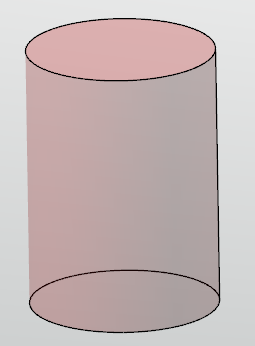
\includegraphics[height=4cm]{bv-cylinder.png}}
  \subcaptionbox{Sphere-shell~包围体\label{fig:subfig-spherical-shell}}
    {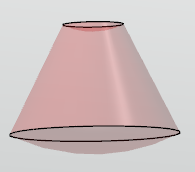
\includegraphics[height=4cm]{bv-spherical-shell.png}}
  \subcaptionbox{圆锥形包围体\label{fig:subfig-bvcone}}
    {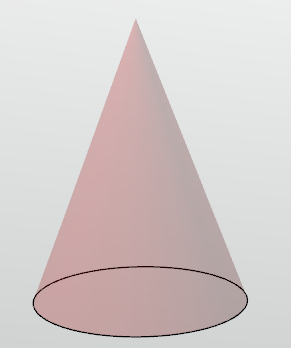
\includegraphics[height=4cm]{bv-cone.png}}
  \\
  \subcaptionbox{椭球形包围体\label{fig:subfig-bv-ellipse}}
    {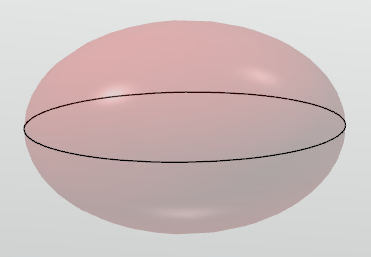
\includegraphics[height=4cm]{bv-ellipse.png}}
  \subcaptionbox{Swept-sphere~包围体\label{fig:subfig-bv-swept-sphere}}
    {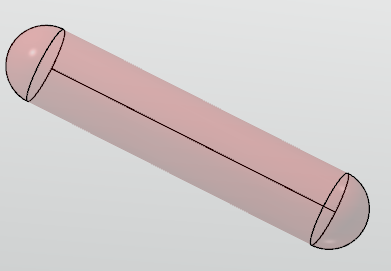
\includegraphics[height=4cm]{bv-swept-sphere.png}}
  \caption{其他包围体}
  \label{fig:bv-others}
\end{figure}

\subsection{包围体的应用}

包围体常见的应用领域有真实感渲染如可见面判别、视域剔除\cite{assarsson2000optimized},光线追踪\cite{wald2007ray}等。
在光线追踪算法中,包围体用于检测光线是否与物体相交,如果光线没有与包围体相交,则肯定不会与包围体内的物体模型相交,进而就不用渲染显示该物体。
另外更常见的应用就是碰撞检测\cite{wangzhiqiang1999},大多数碰撞检测算法都用到了各式各样的包围体以加速,如
\onlinecite{larsson2006dynamic,madera2009hybrid,vogiannou2010enhancing,chang2010efficient,tang2010fast,zhigang2010efficient} 等。

有不少文献将包围体和模型简化技术结合起来,例如~Kai Huebner~等人\cite{huebner2008minimum}在利用文献
\onlinecite{barequet2001efficiently}中提出的构造最小~OBB~包围体算法的基础上将物体分解成多个~OBB~包围体,用这些~OBB~包围体近似原始模型用于机器人抓取中,如图\ref{lbl:Huebner2008-example}所示。
类似的还有~Sphere~包围体的分解\cite{hubbard1996approximating}(如图\ref{lbl:hubbard1996approximating-example}),~Tribox~的分解\cite{crosnier1999tribox}等。

\begin{figure}[H]
  \centering
  \subcaptionbox{模型简化成~OBB~包围体\cite{huebner2008minimum}\label{lbl:Huebner2008-example}}%[3cm] %标题的长度
    {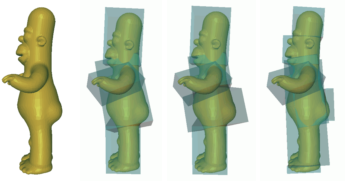
\includegraphics[height=4cm]{Huebner2008-example.png}}
  \subcaptionbox{模型简化成~Sphere~包围体\cite{hubbard1996approximating}\label{lbl:hubbard1996approximating-example}}
    {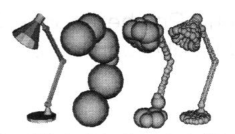
\includegraphics[height=4cm]{hubbard1996approximating-example.png}}
  \caption{包围体应用于模型简化}
  \label{lbl:bounding-voluems-used-in-shape-approximation}
\end{figure}

Jyh-Ming Lien~\cite{lien2006approximate2d}等人在06年提出一种方法可以将给定的多边形(包括含有孔洞的)分解成多个凸多边形,并提供不同种精度的分解,可以应用于~LoD(Level of
Detail,多层次细节)~,并在07年将其扩展到三维\cite{lien2007approximate3d},即提出了一种方法将原始实体模型近似为层次结构的凸包围多面体,如图\ref{lbl:lien2007approximate-example}
所示,对图中的原始模型进行准确凸分解(~ECD,Exact Convex
Decompositions~)将得到726240个组成部分,而近似凸分解(~ACD,Approximate Convex
Decompositions~)仅得到98个组成部分,同时保持了原始模型的大致形状,这大大加速了渲染过程。

\begin{figure}[H]
\centering
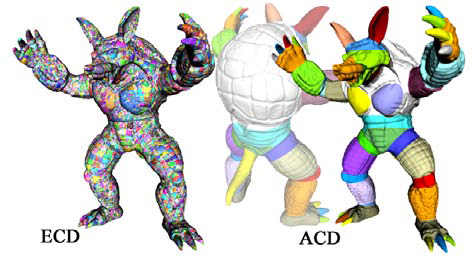
\includegraphics[width=3in]{lien2007approximate-example.png}
\caption{层次结构凸包围多面体的精确构造和近似构造\cite{lien2007approximate3d}}
\label{lbl:lien2007approximate-example}
\end{figure}
这种分解还可以应用于多种应用,例如运动规划(~Motion planning~),网格生成(~Mesh generation~),点定位(~Point location~)问题等等,更多内容可以参考\cite{lien2008approximate} 以及~Jyh-Ming Lien~ 的博士学位论文\cite{lien2006approximatephd}。

文献\cite{attene2008hierarchical}利用一种类似的方法将原始3D模型分解成一个具有层次结构的模型(图\ref{lbl:attene2008hierarchical-example:subfig1}所示),最顶层将是整个模型的凸包。将该算法应用到3D编辑环境中,能够更加方便地让用户选择模型的某个部分进行交互设计。效果如图\ref{lbl:attene2008hierarchical-example:subfig2} 所示,用户选择模型的头部,并进行拖拽能够较快速得到模型新的外观。\footnote{详情可参考视频:http://www.readcube.com/articles/10.1111/j.1467-8659.2008.01271.x }

\begin{figure}[H]
  \centering
  \subcaptionbox{层次结构的分解\label{lbl:attene2008hierarchical-example:subfig1}}
    {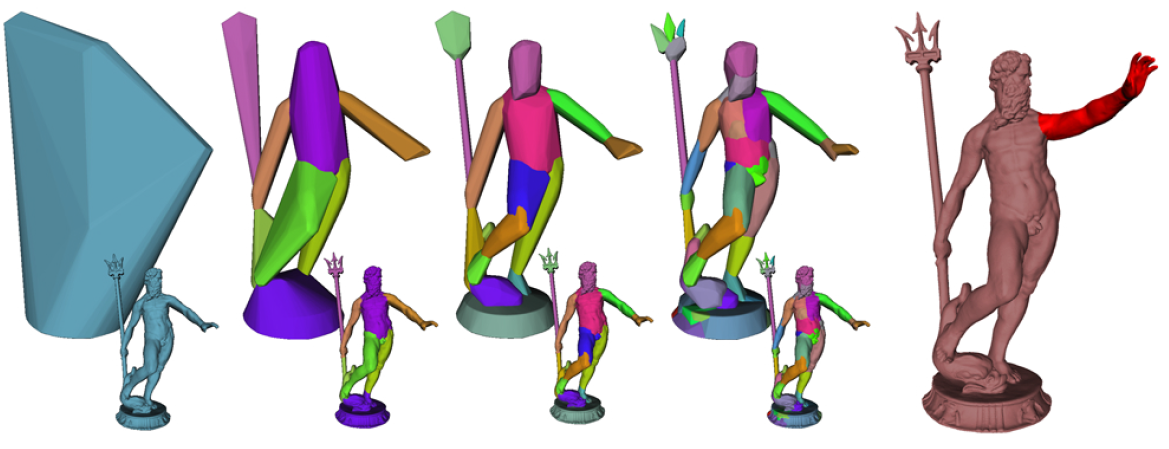
\includegraphics[height=2.8cm]{attene2008hierarchical-example-0.png}}
  \subcaptionbox{区域选择进行交互设计 \label{lbl:attene2008hierarchical-example:subfig2}}
    {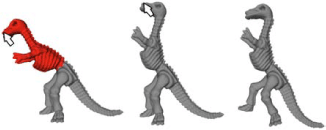
\includegraphics[height=2.8cm]{attene2008hierarchical-example.png}}
  \caption{层次结构的凸包围体及其应用于交互设计\cite{attene2008hierarchical}}
  \label{lbl:attene2008hierarchical-example}
\end{figure}

随着计算机软件技术和硬件的发展,有不少并行算法来计算包围体。
文献\cite{karlsson2010parallel}利用~Intel~单指令多数据流(Single Instruction
Multiple Data~,简称SIMD)~SSE~指令集和~OpenMP~实现了对~AABB~,~OBB~和~$k$-DOP~的计算。
文献\cite{lauterbach2009fast}提出了在~统一计算设备架构(Compute Unified Device
Architecture,简称CUDA,后同)~平台上基于~GPU~构造~AABB~包围体树的方法并应用于光线追踪。

\section{碰撞检测算法}
\label{sec:collisiondetection}

碰撞检测是许多应用的基础,例如在~3D~游戏,物理仿真,机器人,虚拟现实等。本节将就碰撞检测问题的分类和基于包围体树的算法进行阐述。

\subsection{碰撞检测算法的分类}
\label{sec:cd-category}

碰撞检测算法按照不同的分类标准可以有不同的分类方法。
根据其利用的加速结构不同大致可以分为两类,
一类是空间划分树(Spatial Partition Tree~,四叉树,八叉树,~KD~
树等),如文献\onlinecite{Melax2000}就提出了一种基于~BSP~的算法应用于~3D~游戏中的碰撞检测。
另外一种就是层次结构包围体(Bounding Volume Hierarchies
,简称~BVH,也称包围体树),如在\ref{sec:convex-bv}提到的~AABB~,~OBB~等包围体树。
包围体树跟常见的空间划分树最大的区别就是,在~BVH~中的两个或多个包围体可以包含相同的空间,而空间划分树的每个划分结构是分离的,且在~BVH~中,父节点不一定必须完整包含子节点,只需要包含子节点对应原始物体的那部分即可\cite{ericson2005real}。 
根据参与碰撞检测的物体模型的表现形式,又可以分为凸体模型或凹体模型,多边形或者三角网格模型,CSG~(Constructive
Solid Geometry,构造实体几何)模型,隐式方程或者参数表达曲面模型等,例如文献\onlinecite{Zeiller1995}就讨论了计算机动画系统中基于CSG模型的碰撞检测算法,GJK~算法\cite{Science1999}就是针对凸体模型之间的碰撞检测算法。
根据碰撞检测的模拟环境划分,又可以分为成对(Pair
Processing)碰撞检测和多体(Nbody
Processing)碰撞检测,刚体和柔性模型的碰撞检测以及静态和动态(连续)碰撞检测\cite{lin1998collision}。
文献\onlinecite{jimenez20013d}从碰撞检测的解决策略上做了系统的分类和总结,文中提到目前的碰撞检测都是从几何或代数的方法进行求解,其中几何方法主要利用投影、采样或者二者的结合的技术进行处理。

随着~3D~扫描仪的出现,近年来也出现了一些基于点云的碰撞检测算法。Klein Jan~等人\cite{klein2004point}首次在~EuroGraphics 04~上提出了点云的碰撞检测概念,同样利用了层次结构包围体进行加速检测,并提出了一个给定容差的判断点云模型之间是否相交的算法。
文献\cite{figueiredo2010efficient}将~AABB~包围体和~R~树结合起来,并从~OAABB(Overlapped AABB)中找出是否含有一个模型的点在容差范围内逼近另外一个点云模型以此判断是否发生相交。

随着计算机图形卡的产生,又不断涌现出基于~GPU~的碰撞检测并行算法,如文献\onlinecite{Zhang2007Interactive,hebing2009}等,利用~GPU~多线程技术提高碰撞检测的效率。

\subsection{基于包围体树的碰撞检测算法}
\label{sec:cd-bvh}

在第\ref{sec:convex-bv}节中介绍了在对原始几何模型进行求交判断之前先用其包围体判断是否相交有助于提高求交过程的性能,
通过将包围体组织成树形结构即层次结构包围体(BVH)能够将包围体预判阶段从理论上降低到对数时间复杂度(要求树是平衡的)。
当构造原始复杂模型的包围体树时,复杂模型会被拆分成多个部分,每个部分用某种包围体近似,这构成了树型结构的叶子节点,这些节点会按照某种分组策略进行合并成更大的包围体分别构成其父节点,如此递归,最终形成一颗树,树最顶端是一个包含住原始物体的最粗糙的包围体,如图\ref{lbl:bvh-example}
所示,为一个8层~AABB~包围体的~BVH(也可以看作是8层6-DOP的~BVH)。
\begin{figure}[H]
  \centering
  \subcaptionbox*{\label{lbl:bvh-bunny-center-0.png}}
    {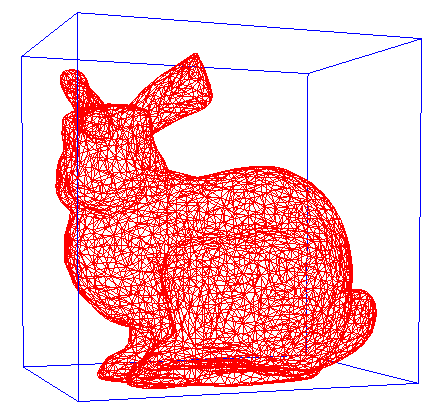
\includegraphics[height=2.8cm]{bvh-bunny-center-0.png}}
  \subcaptionbox*{\label{lbl:bvh-bunny-center-1.png}}
    {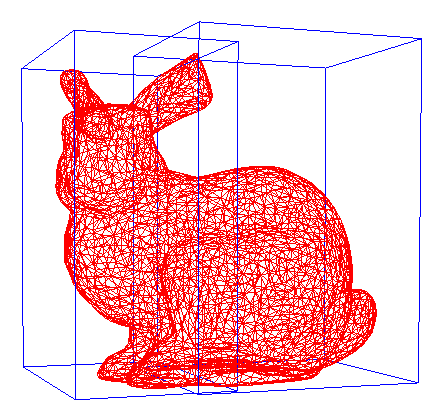
\includegraphics[height=2.8cm]{bvh-bunny-center-1.png}}
  \subcaptionbox*{\label{lbl:bvh-bunny-center-2.png}}
    {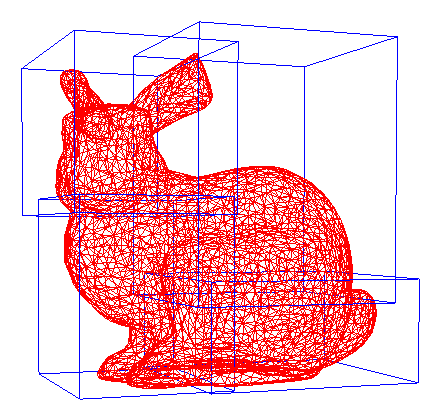
\includegraphics[height=2.8cm]{bvh-bunny-center-2.png}}
  \subcaptionbox*{\label{lbl:bvh-bunny-center-3.png}}
    {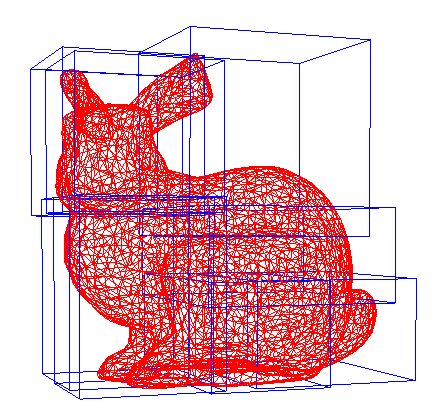
\includegraphics[height=2.8cm]{bvh-bunny-center-3.png}}
    \vspace{-0.3cm}
  \\\hspace{0.5cm} 
  \subcaptionbox*{\label{lbl:bvh-bunny-center-4.png}}
    {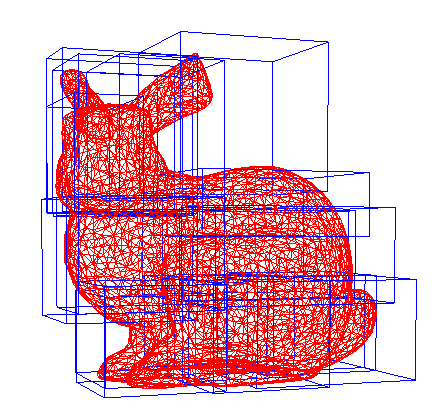
\includegraphics[height=3.0cm]{bvh-bunny-center-4.png}}
  \subcaptionbox*{\label{lbl:bvh-bunny-center-5.png}}
    {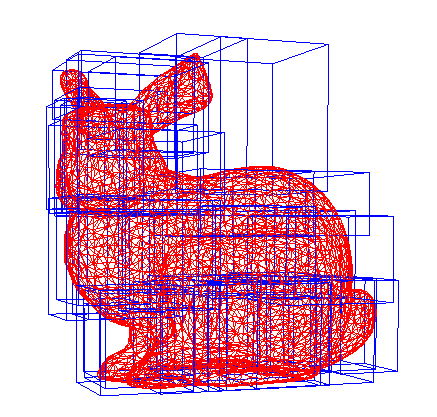
\includegraphics[height=3.0cm]{bvh-bunny-center-5.png}}
  \subcaptionbox*{\label{lbl:bvh-bunny-center-6.png}}
    {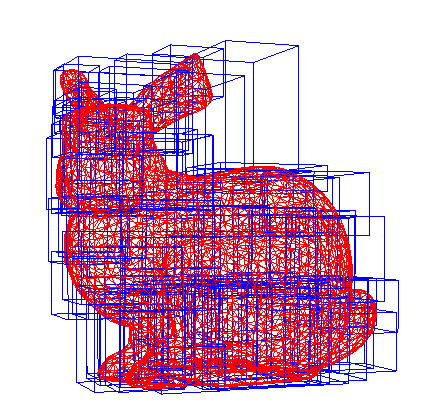
\includegraphics[height=3.0cm]{bvh-bunny-center-6.png}}
  \subcaptionbox*{\label{lbl:bvh-bunny-center-7.png}}
    {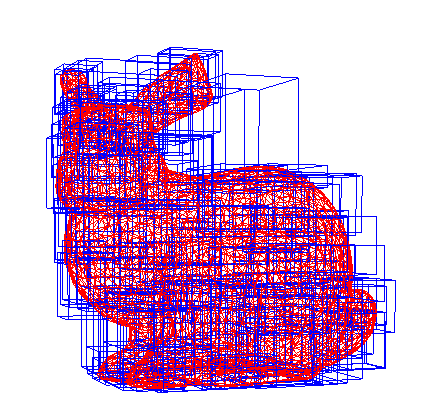
\includegraphics[height=3.0cm]{bvh-bunny-center-7.png}}
\caption{八层~BVH~示例}
\label{lbl:bvh-example}
\end{figure}

在碰撞检测算法中,一般会对模型进行预处理建立起各自的~BVH~树,当两个模型进行相交检测时,自顶向下遍历两棵~BVH~树,若父节点没有相交,则没有必要进行子节点的相交测试,自顶向下的遍历算法如算法~\ref{alg:traverse-bvh-tree}~所示。

\begin{algorithm}
\algsetup{linenosize=\tiny}
\small
\caption{$TraverseBVHTree(node_1, node_2)$}
\label{alg:traverse-bvh-tree}
\begin{algorithmic}[1]
\REQUIRE
$node_1$,$node_2$:BVH~树中的节点1、节点2
\ENSURE
是否相交
\IF{$node_1.bv \cap node_2.bv = \emptyset$} 
    \RETURN \FALSE \COMMENT{包围体重合测试, 包围体不相交直接返回}
\ELSE
    \IF {$node_1.children = \emptyset$}
         \IF {$node_2.children = \emptyset$}
            \RETURN {$CheckIntersection(node_1.primitives, node_2.primitives)$}
            \COMMENT{最底层叶子节点原生几何相交测试}
         \ELSE
            \FORALL {$child \in node_2.children$}
                \STATE $TraverseBVHTree(node_1, child)$ \COMMENT{递归调用}
            \ENDFOR
         \ENDIF
    \ELSE
         \FORALL {$child \in node_1.children$}
            \STATE $TraverseBVHTree(child, node_2)$  \COMMENT{递归调用}
         \ENDFOR
    \ENDIF
\ENDIF
\end{algorithmic}
\end{algorithm}

从算法~\ref{alg:traverse-bvh-tree}~可以看出,基于~BVH~的碰撞检测算法性能的好坏关键在于两个操作,一是分别来自两个~BVH~内部节点包围体之间的相交测试,二是~BVH~最底层叶子节点内的原生几何相交测试,常常利用~$T_{cost}
= n_v * C_v + n_p * C_p$ 来衡量单个相交测试的所付出的代价,其中$n_v$
和$n_p$分别表示参与包围体节点相交测试的数量和参与原始几何相交测试的数量,$C_v$和$C_p$则表示相应的平均测试耗费的代价\cite{klosowski1998efficient}。
当运动场景或连续碰撞的模型之间的碰撞检测时,往往还需要考虑到因物体模型旋转平移等变换产生的包围体的更新所付出的代价,即上述代价函数变成$T_{cost}
= n_v * C_v + n_p * C_p + n_u *
C_u$,要提高碰撞检测的性能,就得想办法减小$T_{cost}$的值。本文的算法主要关注于静态场景。

不同的包围体,上述代价函数各个值不同,对于不同的应用场景,可能需要选择不同的包围体进行加速碰撞检测。
文献\onlinecite{zhigang2010efficient}从包围体的构造难度,包围体的紧致性,包围体之间相交测试复杂性及包围体在运动过程中的更新代价几个方面对五种常见的包围体进行了比较,如表\ref{lbl:table:bv-comp}所示。
可以看出,各种包围体有各自的优缺点和适用场景,因此,很多研究人员充分利用各种包围体的优点,将多种包围体结合在一起组成新的组合包围体。
文献\cite{chang2010efficient}利用~OBB~包围体相对的紧致优点和球形包围体相交测试简单性的优点进行组合,构造~OBB-Sphere~包围体,在进行相交测试时,先利用球形包围体进行测试,如果相交再用~OBB~进行测试。
类似的,文献\cite{zhigang2010efficient}同时利用更加紧致的$k$-DOP~和~Sphere~包围体构造$k$-DOP-Sphere~包围体。

\begin{table}[H]
\centering
\caption{碰撞检测中常用凸包围体比较}
\begin{tabular*}{13cm}{ccccc}
\toprule[1.2pt]
凸包围体 & 构造代价 & 相交测试简单性 & 紧致性 & 更新代价\\
\midrule[1pt]
AABB   & 1 & 2 & 4 & 3\\
OBB    & 4 & 4 & 3 & 2\\
Sphere & 2 & 1 & 5 & 1\\
k-DOP  & 3 & 3 & 2 & 4\\
Convex hull & 5 & 5 & 1 & 5 \\
\bottomrule[1.2pt]
\end{tabular*}
\label{lbl:table:bv-comp}
\end{table}


\section{本文主要内容}
\label{sec:structure}
本文着重讨论如何快速地生成紧致性可控的凸包围体以及将此包围体应用于静态场景的碰撞检测。
第一章首先介绍了当前各种凸包围体的特征及应用。然后再介绍了碰撞检测问题的背景和本文研究的基于凸包围体的碰撞检测算法。

第二章提出了紧致性可控的凸包围体$k$-CBP($k$-Convex Bounding Polyhedron)~的生成算法,紧致性可控主要通过凸包围体的平面数量$k$来调节。
该算法法首先利用近似内凸包和~$k$-means~聚类算法生成构成凸包围多面体~$k$~个截面的法向,
然后根据输入点集沿各法向搜索切点构成截面,最后由这些截面通过对偶映射的方式求交构成凸包围多面体。
在搜索截面过程中,提出了两种并行策略以加速搜索过程。实验结果表明,与同类算法相比,该方法能够更快地构造给定点集更紧致的凸包围多面体。

第三章提出了基于本文提出的$k$-CBP~包围体的碰撞检测算法,在包围体之间的相交测试时分别用~AABB~树的方式和基于~GJK~算法的两种方式进行。
实验结果表明本文提出的凸包围体能够有效加速碰撞检测算法。

第四章是对本文的研究工作进行总结,以及未来可以改进的方向。


%%% Local Variables: 
%%% mode: latex
%%% TeX-master: t
%%% End: 

\chapter{凸包围体生成算法}
\label{cha:kcbp-construction}
从第~\ref{sec:convex-bv}~节可以看出包围体的紧致程度直接影响相应算法的效率,对于不规则形体, 常见的包围体往往不够紧致,凸包紧致但往往包含过多的面片数而增加算法的复杂性。

本文提出一种构造凸包围多面体的方法,该方法首先利用近似内凸包和~$k$-means~聚类算法生成构成凸包围多面体~$k$~个截面的法向。
然后根据输入点集沿各法向搜索切点构成截面, 最后由这些截面通过对偶映射的方式求交构成凸包围多面体。搜索截面过程中,各个法向的搜索过程相互独立互不影响,因此可以方便地利用~GPU~进行加速。
本文提出的方法的主要优势是:
\begin{inparaenum}[(1)]
\item 对给定点集可构造紧致的包围体;
\item 利用~GPU~加速,能够快速构造包围体;
\item 通过参数~$k$~调节凸包围多面体的简单性和紧致性,可适用于不同的应用场景。
\end{inparaenum}

由~$k$~个截面构成的凸包围多面体称为凸包围~$k$~面体($k$-Convex Bounding Polyhedron,简称~$k$-CBP), 可通过~$k$~个半空间定义:
\begin{equation}
\label{equ:kcbp_definition}
\left\{
\begin{array}{l}
    k\mbox{-CBP} = \mathop  \bigcap \limits_{i = 1}^k \bm{H_i} \\
    \bm{H_i} = \left\{ {\left. {\bm{p} \in {\mathbb{R}^3}} \right| \bm{n_i} \cdot \bm{p} \le {w_i}} , w_i \in \mathbb{R} \right\},
\end{array}
\right.
\end{equation}
其中,$\bm{n_i}$~是半空间~$\bm{H_i}$~的法向,方向指向包围体外部,
$w_i$~是输入点集中沿~$\bm{n_i}$~方向投影的最大值。
如图~\ref{fig:bunny}~所示是~Bunny~模型的凸包围~34~面体(34-CBP)。

\begin{figure}[htbp] 
\centering
  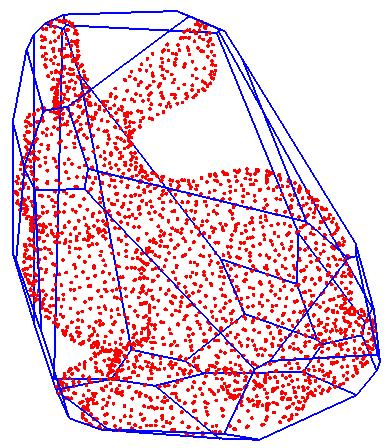
\includegraphics[width=1.5in]{bunny-34.png}
  \caption{~Bunny~模型的~34-CBP }
  \label{fig:bunny}
\end{figure}

本文算法的主要流程如图~\ref{lbl:kcbp-algorithm-flowchart}~所示,首先利用近似内凸包和~$k$-means~聚类算法生成构成凸包围多面体~$k$~个截面的法向,然后根据输入点集在~GPU~中沿各法向搜索切点构成截面,
最后由这些截面通过对偶映射的方式求交构成凸包围多面体。搜索截面需要多次扫描输入点集,在~CPU~中计算较耗时,因此用~GPU~加速使得算法整体性能得以提升,其他步骤在~CPU~计算即可。

\begin{figure}[htbp]
    \centering
    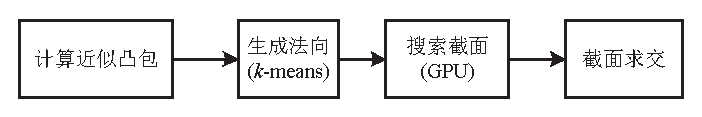
\includegraphics[width=5.5in]{kcbp-flowchart-x-aix.eps}
    \caption{构造~$k$-CBP~算法流程图}
    \label{lbl:kcbp-algorithm-flowchart}
\end{figure}

图~\ref{lbl:bunny-26-cbp-ch-ach}~从左至右分别显示了~Bunny~模型的~26-CBP、精确凸包和近似内凸包。
近似凸包是精确凸包的一种近似,与精确凸包外观相似但其构造复杂度降低,不少研究者利用该性质解决计算机图形学中很多问题\cite{hossain2013constructing}。

\begin{figure}[htbp] % use [htbp] to fix the position
\centering
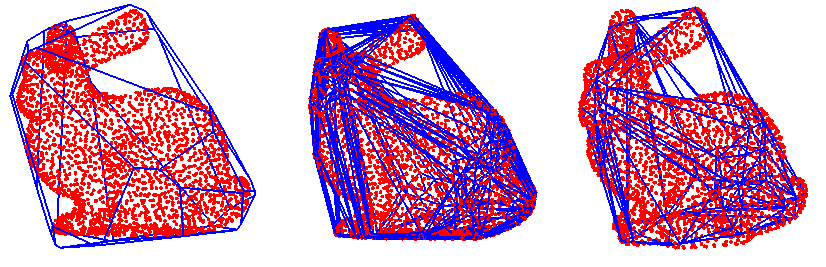
\includegraphics[width=5.0in]{26-bunny-ach-ch-kcbp.png}
\caption{~Bunny~模型的~26-CBP、凸包和近似内凸包}
\label{lbl:bunny-26-cbp-ch-ach}
\end{figure}

本文就利用了近似内凸包与精确凸包的相似性,从众多近似凸包面片的法向中通过~$k$-means~聚类算法生成构成凸包围多面体的~$k$~个法向。
本章后续部分将按步骤详细介绍算法的实现。
%由图可知, 近似内凸包的三角面片大致反映了精确凸包三角面片的分布情况,近似内凸包相应位置面积较大的三角面片对应到精确凸包的三角面片面积也较大, 因此该三角面片所在平面需尽量保留.

\section{截面法向的生成}
\label{sec:gen-normals}

截面法向的选定与多面体的紧致程度密切相关。
$k$-DOP\cite{klosowski1998efficient}~预先定义~$k/2$~对法向,且~$k$~值局限于6、14、18或26等少数几个,对于不同的模型其方向始终一致,导致其生成的多面体不能自适应模型,对于不规则形体的模型不够紧致。
与~$k$-DOP~相比,本文算法~$k$~值取值更灵活,因此可以根据不同需求不同应用场景更加灵活地选择需要的凸包围体。
根据经验,为了使凸包围多面体尽可能逼近凸包,在多面体数量一定的情况下需尽量保留凸包中面积较大的面。 
本文生成凸包围多面体的法向的流程是先通过一种线性算法\cite{bentley1982approximation}构造近似内凸包,然后从近似内凸包里选取面积最大的~$a$~个面的法向,最后用聚类算法从剩下的面中生成~$k-a$~个法向。
下面将介绍截面法向生成的主要步骤。

\subsection{近似内凸包生成聚类样本法向集}
\label{subsec:ach-gen-normals}

以平面点集的近似内凸包为例说明初始法向集的生成。

\begin{figure}[htbp]
  \centering
  \subcaptionbox{分组\label{lbl:subfig-split-groups}}{
    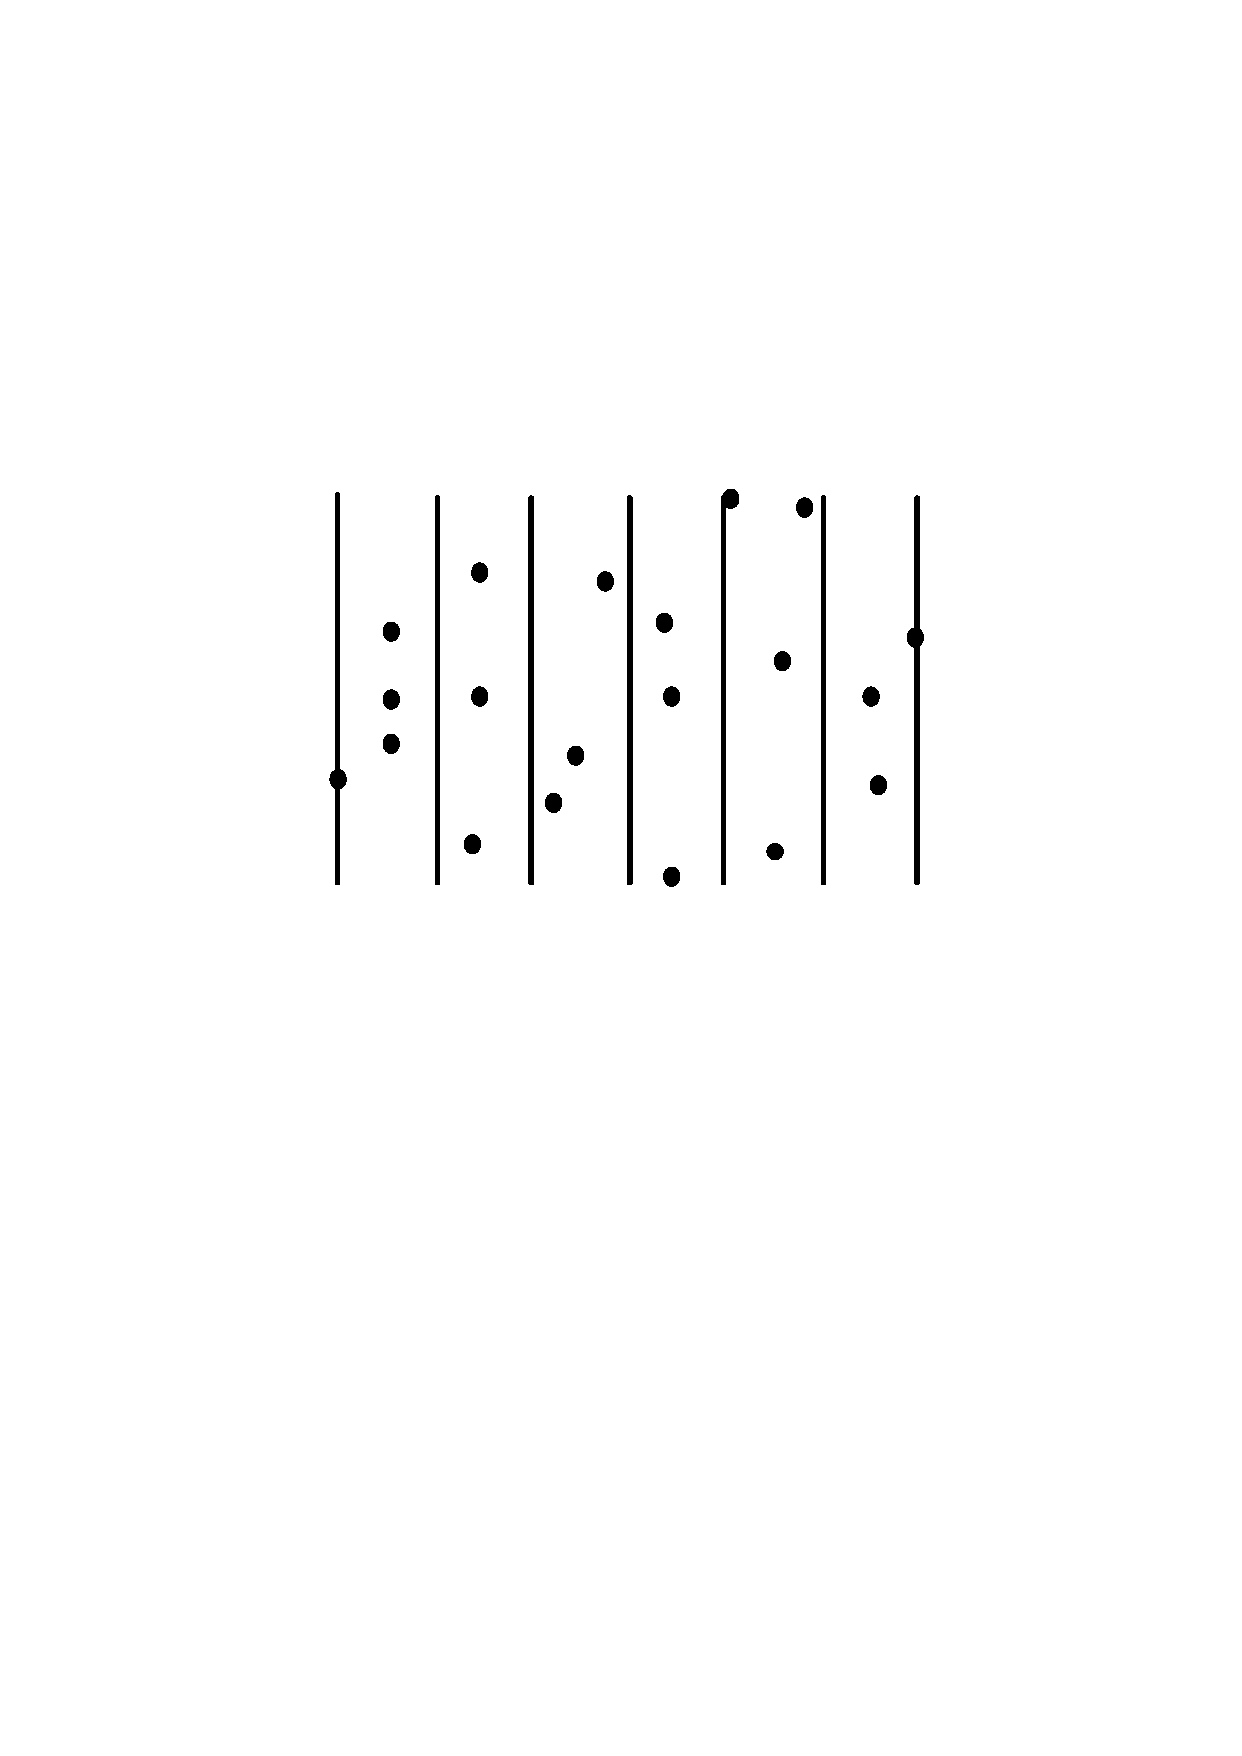
\includegraphics[width=2.2in]{approximate-convexhull-step1.pdf}} \hspace{0.5cm}
  \linebreak
  \subcaptionbox{选极值点\label{lbl:subfig-find-extrems}}{%
    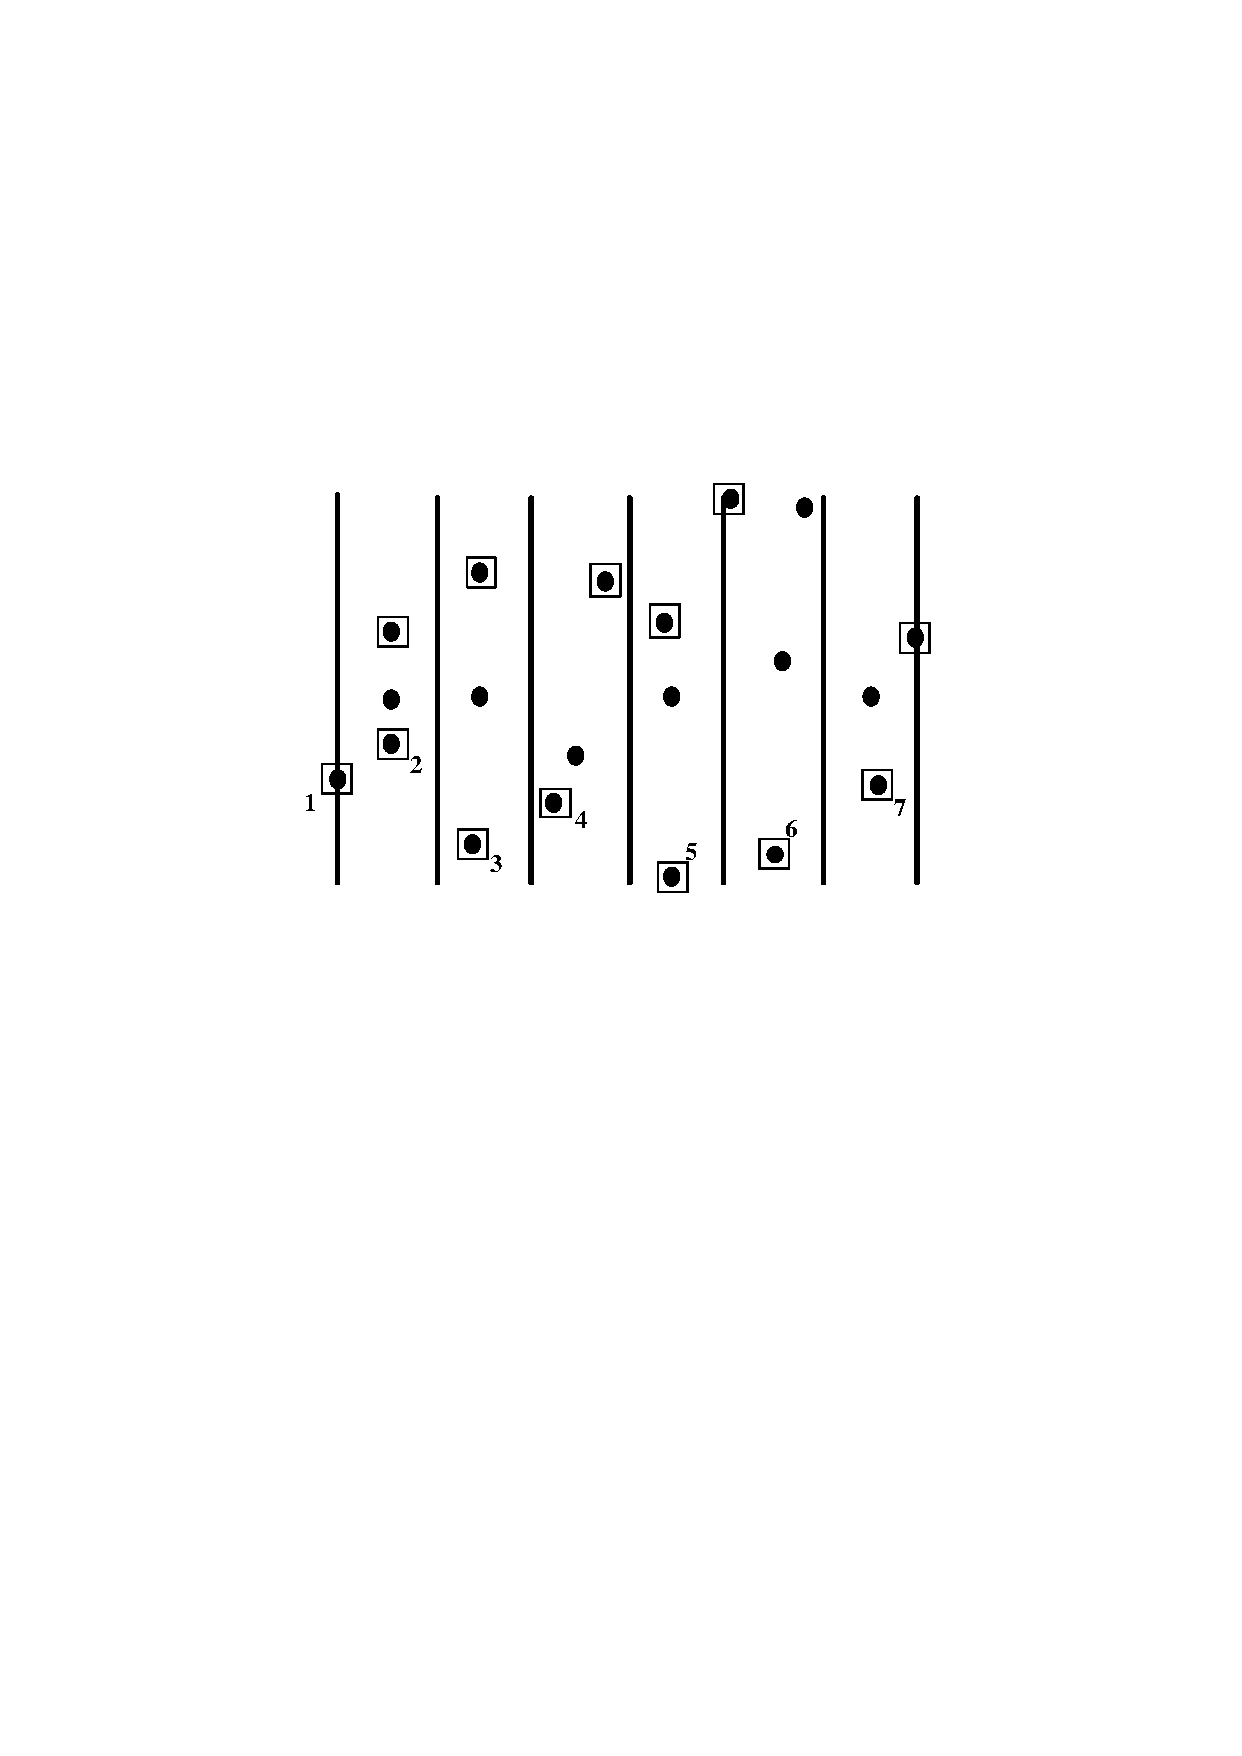
\includegraphics[width=2.2in]{approximate-convexhull-step2.pdf}} \hspace{0.5cm}
  \hspace{2em}
  \subcaptionbox{连线\label{lbl:subfig-connect-extremes}}{%
    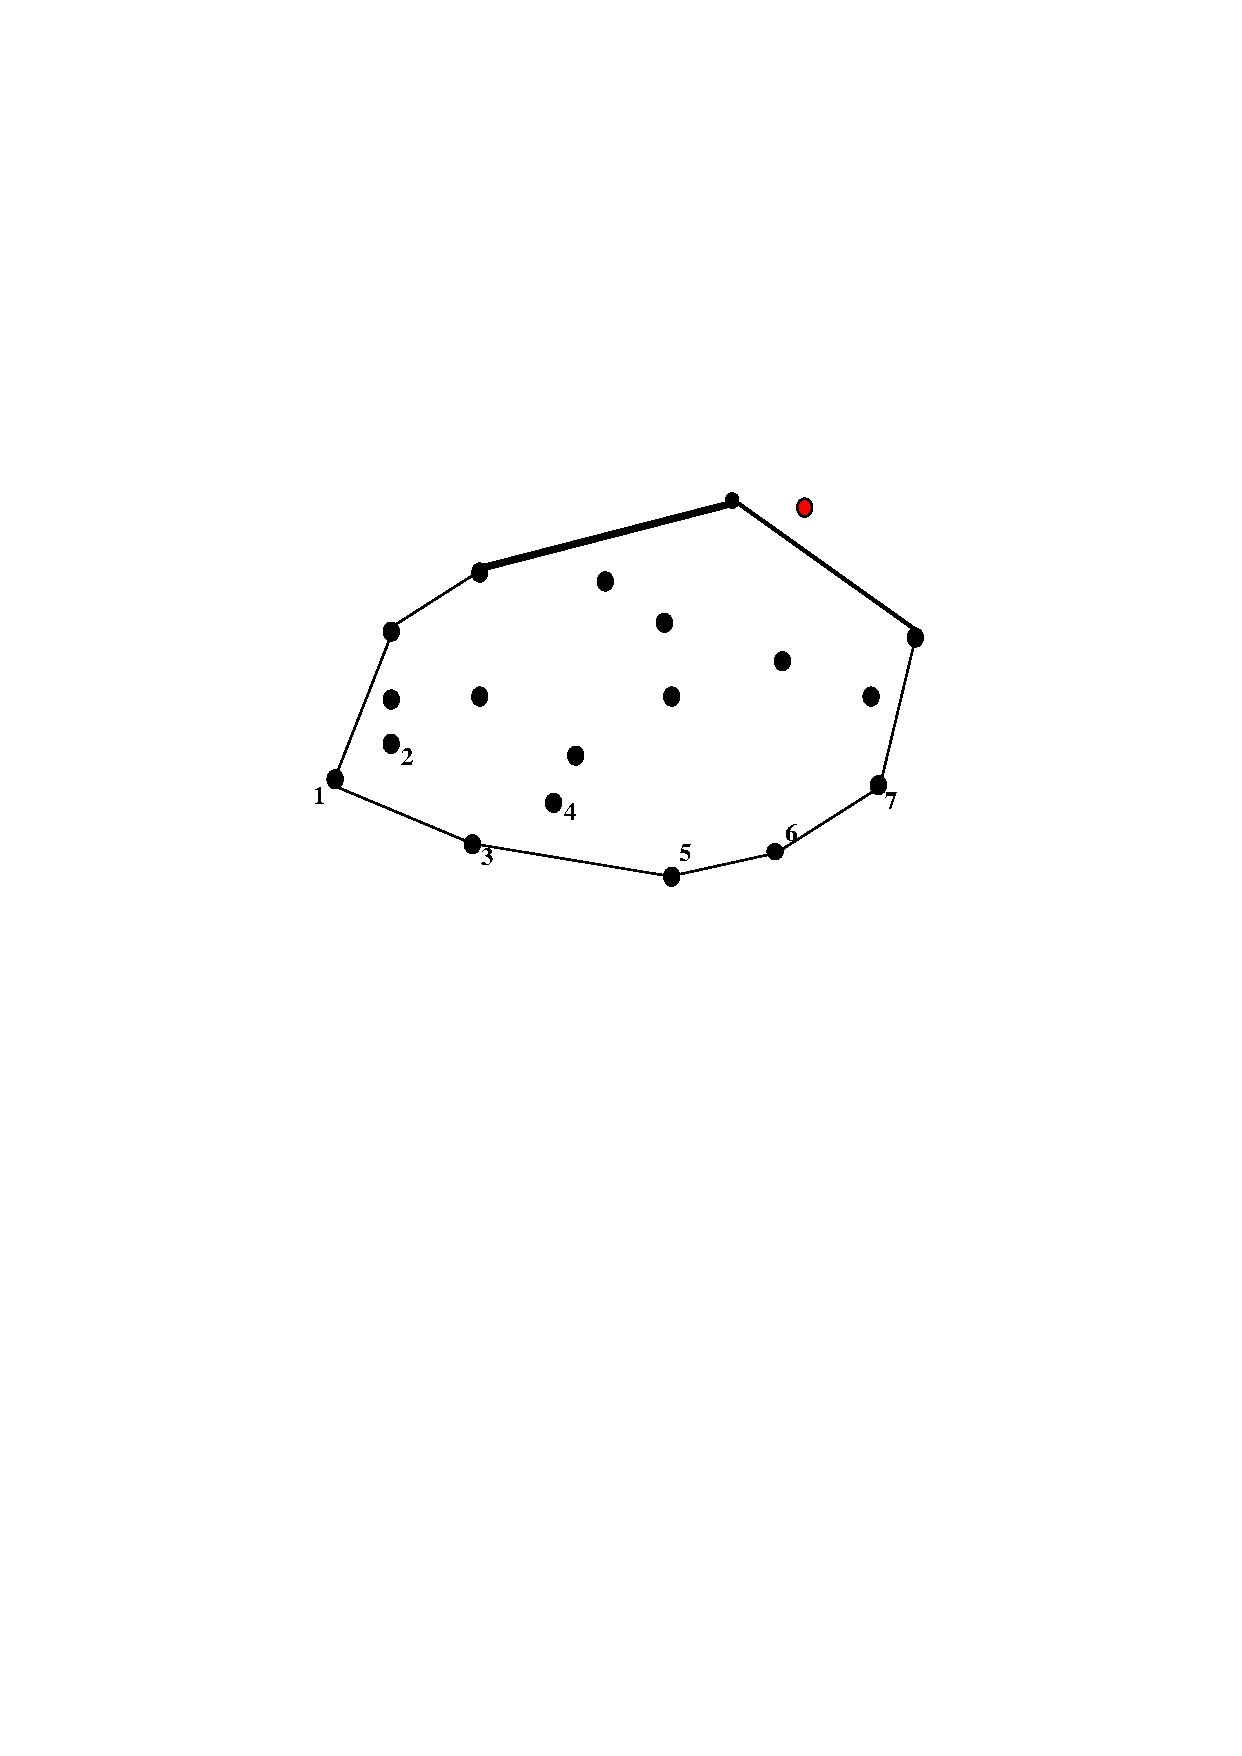
\includegraphics[width=2.2in]{approximate-convexhull-step3.pdf}} \hspace{0.5cm}
  \caption{二维近似内凸包的构造\cite{bentley1982approximation}}
\label{lbl:ach-2d}
\end{figure}

如图~\ref{lbl:ach-2d}~所示,整个算法分为如下3个步骤:

\begin{inparaenum}[(1)]
%\begin{enumerate}[(1)]
\item \textbf{分组:}
首先根据~$x$~轴将输入点集均分~$\xi$~组,如图~\ref{lbl:subfig-split-groups}所示,$\xi$值可以根据输入点集数量以及希望得到的近似凸包的近似程度进行选取,图示中分成了~6~组。\\
\indent \item \textbf{选极值点:}
然后在每组中找出沿~$y$~轴的最大最小坐标值的点,得到每组的极值点,如图~\ref{lbl:subfig-find-extrems}~所示,在边界上的点可直接当作极值点。\\
\indent \item \textbf{连线:}
最后按条件连接每组的最值构成近似内凸包,如图~\ref{lbl:subfig-find-extrems}所示,以下半圈为例,在选定的极值点中先选定最左边的点~1,下一个候选点~2,连接~13~发现候选点~2~在~13~的左边,丢弃候选点~2~直接连接~13,同理连接~35,
当查看候选点~6~时,发现点~6~在~57~连线的右边,因此候选点~6~保留,依次类推可得整个下半圈为凸包,上半圈同理可得。最后合并上下半圈得到如图~\ref{lbl:subfig-connect-extremes}所示的结果。
\end{inparaenum}
%\end{enumerate}

此算法复杂度为~$O(n+\xi)$。  
得到近似凸包后,因较长的边(图~\ref{lbl:subfig-connect-extremes}~中的粗边)对最后凸包围多边形影响较大, 因此可以保留较长的~$a$~条边, 其他~$n-a$($n$~为近似内凸包边数)进行聚类得到~$k-a$~类, 最后得到边对应的垂直向外的方向作为法向。
在三维空间里, 可按照~$x,y$~轴最多划分成~$(\xi+2)\times (\xi+2)$~个正方体网格, 每个正方体网格取~$z$~轴的最大最小坐标值, 因此所有网格含最多含有~$2(\xi+2)^2$~个极值点, 其凸包可以在~$O(\xi^2\log \xi^2) = O(\xi^2\log \xi)$~内求得, 因此整个算法时间复杂度为~$O(n+\xi^2\log\xi)$, 
关于此算法更详细的细节可参考文献~\onlinecite{bentley1982approximation}。 实验过程中, 为了更快地构造近似内凸包, $\xi$~值通常取得较小(例如取~$\xi=10$)。

假设点~$A,B,C$~为近似凸包的某个平面~$P_i$~上逆时针方向上的3个顶点,则该平面~$P_i$~的法向~$\bm{n_i}
= \overrightarrow{AB} \times
\overrightarrow{AC}$,这些法向就是参与聚类算法的所有样本法向集。

\subsection{聚类初始点的选择}
\label{subsec:initial-normals}

聚类算法是数据挖掘领域里的研究热点之一,$k$-means~是最流行和最简单的基于划分的聚类算法\cite{Jain2010}。其中,$k$-means
算法最初的步骤就是初始聚类中心的选择。本文算法将采取如下的策略生成:给定一个单位球,将其按照等面积划分成$k$份即$k$-means中的参数$k$,连接球心到每份中心点构成的方向作为法向,其效果如图~\ref{lbl:kmeans-init-normals-26}~所示($k=26$)。

\begin{figure}[htbp]
    \centering
    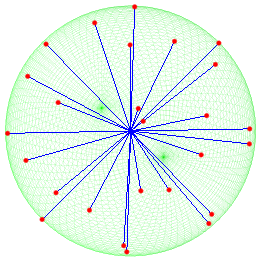
\includegraphics[height=1.7in]{kmeans-init-normals-26.png}
    \caption{初始聚类法向的生成}
    \label{lbl:kmeans-init-normals-26}
\end{figure}
初始点生成算法具体如算法~\ref{alg:get_init_normals_by_area}~所示\footnote{http://www.cmu.edu/biolphys/deserno/pdf/sphere\_equi.pdf}。
另外,亦可使用如文献~\onlinecite{wong1997sampling}~中的数学统计方法在球面上生成若干个点使其满足均匀分布。

\begin{algorithm}[htbp]
\small
\caption{初始法向的生成}
\label{alg:get_init_normals_by_area}
\begin{algorithmic}[1]
\Require
初始法向数量~$k$
\Ensure
$k$~个法向~$normals$

\Function{GenerateInitNormal}{$k$}
  \State $area \leftarrow 4\pi / k$
  \State $m\_v \gets \Call{round}{\pi/\sqrt{area}}$
  \State $d\_v \gets \pi/m\_v$
  \State $d\_phi \gets area/d\_v$
  \For {$m=0 \to m\_v-1$}
      \State $v \gets \pi m/m\_v$
      \State $m\_phi \gets \Call{round}{2\pi\sin{v}/d\_phi}$
      \For {$n=0 \to m\_phi-1$}
          \State $\phi \gets 2\pi n/m\_phi$
          \State $normals \gets normals \cup \Call{vec3}{\sin{v}\cos{\phi},\sin{v}\sin{\phi},\cos{v}}$
      \EndFor
  \EndFor
  \State \Return $normals$
  \EndFunction
\end{algorithmic}
\end{algorithm}
 
\subsection{聚类确定法向}
\label{subsec:determ-normals}

聚类算法将相似程度高的变量聚集到一类,距离度量是$k$-means中的关键,采用不同的距离计算函数可能得到不同的聚类结果,依据数据的不同性质可选用不同的距离度量方法,常用的有欧式距离,曼哈顿距离和卡方距离等等。
本文采用余弦距离度量,将方向相近的点归聚到一类。$k$-means~本质上是一个迭代贪心算法,每一次迭代需要重新计算每一类的中心点,直到两次迭代后中心点相差在给定的容差范围内为止。
完整的算法如算法~\ref{alg:kmeans-determine-normals}~所示。

\begin{algorithm}
\small
\caption{$k$-means~确定法向}
\label{alg:kmeans-determine-normals}
\begin{algorithmic}[1]
\Require
初始中心点~$init$, 聚类数量~$k$, 聚类样本法向集~$points$
\Ensure
~$k$~个聚类后的法向 $result$
\Function{kmeansCluster}{$init, k, points$}
  \ForAll {$p \in points$}
    %\State $tmp \gets -\infty $
    \ForAll {$c \in init$}
        \State $\phi \gets c \cdot p$ \Comment{计算余弦距离, 并记录每个聚类变量属于哪一类}
        %\State $tmp \gets max(tmp, \phi)$ \Comment{记录每个聚类变量属于哪一类}
    \EndFor
    \ForAll {$c \in init$}
    \State $result \gets \Call{Update}{c}$ 
        \Comment{按照公式(\ref{equ:kmeans-update-center})更新中心点}
        \State \Comment{检测继续迭代条件是否满足,中心点容差范围内不再变化或迭代次数超过最大迭代次数}
        \If{$ \Call{checkState}{result, init, iter}$}
        \State \Return {$result$}
    \Else
        \State $init \gets result $
        \State $iter \gets iter+1 $
    \EndIf
    \EndFor
  \EndFor
\EndFunction
\end{algorithmic}
\end{algorithm}

算法~\ref{alg:kmeans-determine-normals}~中第7行~\textproc{Update}~方法作用是聚类迭代更新每类的中心点,
本文更新中心点时将每个法向对应的面片的面积作为权重即
\begin{equation}
\label{equ:kmeans-update-center}
\bm{c_i}=\frac{\sum_{i=1}^{i=n} \omega_i \cdot \bm{n_i} } {\sum_{i=1}^{i=n} \omega_i}
,
\end{equation}
其中,$\bm{c_i}$~为第~$i$~类的中心点,$\omega_i$~为法向~$\bm{n_i}$~所在面片对应的面积,这样使得生成的法向尽量靠近原始近似凸包面积较大的面片的方向。

通过用聚类方法得到的法向生成的凸包围多面体比直接用初始法向生成的包围体更加紧致。
如图~\ref{lbl:kemans-fixed-kcbp}~所示, 
其中图~\ref{lbl:fixed-kcbp-bunny}~为按照初始方向为~Bunny~模型生成的凸包围多面体,其中~$k=26$。
聚类后其法向及其生成的凸包围多面体如图~\ref{lbl:kmeans-kcbp-bunny}~所示,后者的紧致程度比前者高~14.98\%。

\begin{figure}[htbp]
\setcounter{subfigure}{0}
  \centering
  \subcaptionbox{初始法向生成$k$-CBP\label{lbl:fixed-kcbp-bunny}}{%
    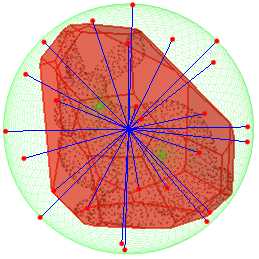
\includegraphics[width=1.8in]{kmeans-init-normals-26-for-bunny.png}}\hspace{3em}%
  \subcaptionbox{聚类法向生成$k$-CBP\label{lbl:kmeans-kcbp-bunny}}{%
    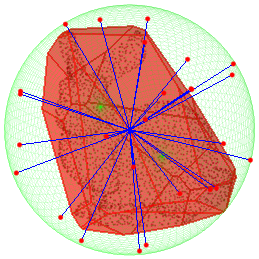
\includegraphics[width=1.8in]{kmeans-cluster-normals-26-for-bunny.png}}\hspace{3em}%
  \caption{初始法向和聚类确定法向生成$k$-CBP对比($k=26$)}
  \label{lbl:kemans-fixed-kcbp}
\end{figure}

\section{搜索截面}
\label{sec:search:planes}

在确定构成~$k$-CBP~的法向后,只需要搜索空间上的一个点即可确定
~$k$-CBP~的截面,搜索截面等效于寻找沿着法向上的最大投影值,即对每个法向~$\bm{n_i}$,从输入模型的所有点中寻找最大投影值的点作为切点进而确定法向~$\bm{n_i}$~对应的截面。
具体算法如算法~\ref{alg:search-plans-cpu}~所示,算法输入为第~\ref{sec:gen-normals}得到的截面法向~$normals$~和模型所包含的点集$points$,算法结束返回多面体的截面~$planes$,
每个截面都是由法向和沿该法向上最大投影值的点构成的,该过程的时间复杂度为~$O(k\cdot n)$,其中~$k$~为法向数量,$n$~为模型点的数量。

\begin{algorithm}[htbp]
\small
\caption{搜索截面串行算法}
\label{alg:search-plans-cpu}
\begin{algorithmic}[1]
\Require
截面法向~$normals$, 模型点集~$points$
\Ensure
多面体截面 $planes$
\Function{SearchCuttingPlanes}{$normals, points$}
  \ForAll {$\bm{n} \in normals$}
      \ForAll {$\bm{p} \in points$}
          \State $proj \gets  \bm{p} \cdot \bm{n}$ \Comment{计算投影值}
          \State $max\_proj \gets \Call{max}{proj, max\_proj}$ \Comment{更新最大投影值}
      \EndFor
  \EndFor
  \ForAll {$\bm{n} \in normals$}
      \State $max\_point \gets \bm{n} \cdot max\_proj$ \Comment{切点}
      \State $planes\gets planes \cup \Call{plane}{\bm{n}, max\_point}$ \Comment{构造平面}
  \EndFor
  \State \Return $planes$
\EndFunction
\end{algorithmic}
\end{algorithm}

从算法~\ref{alg:search-plans-cpu}~可以看出该搜索过程中各法向的计算相互独立,互不影响,因此可方便地借助~GPU~并行加速。
本文将采用着色器和基于~GPU~的通用计算框架两种较流行的并行平台进行~GPU~加速,具体而言为基于~OpenGL~着色语言和~CUDA~框架,下面将分别介绍这两种平台的实现。

\subsection{基于着色器的并行算法}
\label{subsec:determ-normals-by-shader}

OpenGL~提供了可编程管线,它的轻便性、跨平台性和被广泛硬件厂家所支持使得~OpenGL~着色语言(OpenGL Shading Language,简称~GLSL)被广泛应用,在基于~GPU~的通用计算(General
Purpose Graphic Process Unit,简称~GPGPU)中也发挥着重要作用。下面将分别介绍本文提出的基于深度缓冲(Z Buffer)和乒乓技术的算法。

\subsubsection{基于深度缓冲的算法}
	
在~OpenGL~中,当渲染~3D~模型时,深度测试是在片段着色器工作后的一个重要测试操作,当两个片段在相同的位置时,深度测试的目的是决定哪个片段将要保留下来,默认情况下,最前面即有较小(或较大,可设置)的~$z$~坐标值的片段将通过测试被保留下来。
每个片段的深度信息保存在深度缓冲中,当新的片段通过测试后将更新缓冲中的值。
本文充分利用了~OpenGL~的这种机制,算法每走一遍渲染流程将找出一个方向上的切点,在顶点着色器中,将所有点的~$x,y$~坐标值设为一样,并将该点在法向上的投影作为~$z$~值即深度值,所有点经过深度测试后将只有~$z$~值最大的点被保留下来,该点就是沿着这个法向的切点。该过程的算法流程图如~\ref{fig:flowchart:zbuffer}~所示。

\begin{figure}[htbp]
  \centering
  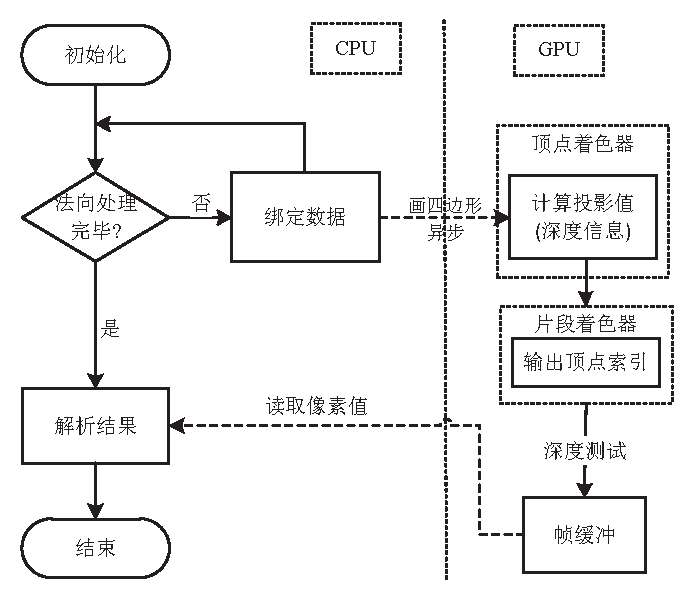
\includegraphics[width=4.0in]{shader-z_buffer.eps}
  \caption{基于~Z Buffer~算法流程图}
  \label{fig:flowchart:zbuffer}
\end{figure}

在实际实现过程中需要注意默认情况下~OpenGL~处理~$x$~和~$y$~坐标值的范围是~$[-1,1]$,而深度值需要映射到~$[0,1]$。我们利用一张~$k \times 1$~大小的纹理保存结果,将第~$i$~个法向的切点保存在纹理的~$(i,0)$~坐标处,
这样做的好处是每绘制一遍不用清除深度缓冲,最后可以一次性读取这个~$k \times 1$~大小的纹理得到结果。
如代码~\ref{shader:zbuffer}~的着色器代码所示,OpenGL~中利用齐次坐标处理渲染流程,因此我们利用前三个分量保存法向的~$x,y,z$~坐标值,第4个分量~$w$~保存法向的索引,在片段着色器中,只需要简单地输出切点的在输入点数组的索引即可。
通过绘制~$k$~遍,我们从大小为~$k \times 1$~的纹理中读出点索引以此就能确定~$k$~切平面,每绘制一遍得到1个切平面,当~$k$~值较大时,这个过程仍然比较耗时,从实验结果也能看出,这种算法适用于~$k$~值相对较小的情况。
%\lstinputlisting[language={shader}, caption={Vertex shader(Z buffer algorithm)}, label=vertex_shader_zbuffer]{shader_zbuffer.vert}
\lstinputlisting[language={shader}, caption={基于~Z Buffer~算法着色器代码}, label=shader:zbuffer]{shader_zbuffer.vert}

\subsubsection{基于乒乓技术的算法}

渲染到纹理(Render To Texture,简称~RTT)是一个非常重要的图形可视化技术,它能够帮助快速地渲染很多漂亮的结果,同时也是~GPGPU~重要组成部分。在基于~OpenGL~的~GPGPU~中,通常要将参与计算的数据通过~CPU~传送至~GPU~的特定大小的纹理中,
通过绘制一个与保存数据有着同样大小的四边形来调用着色器中的算法\cite{gpgpuqiu},将结果输出到纹理中。该过程中,绘制同样大小的四边形是为了避免纹理插值对输入数据的影响。
RTT~的算法一般是在片段着色器(Fragment Shader)中完成,有时通过一遍的绘制得不到最终结果还需要把前一次运算结果传递给下一次运算用来作为后继运算的输入,此时可以利用乒乓技术来解决。

\begin{figure}[htbp]
  \centering
  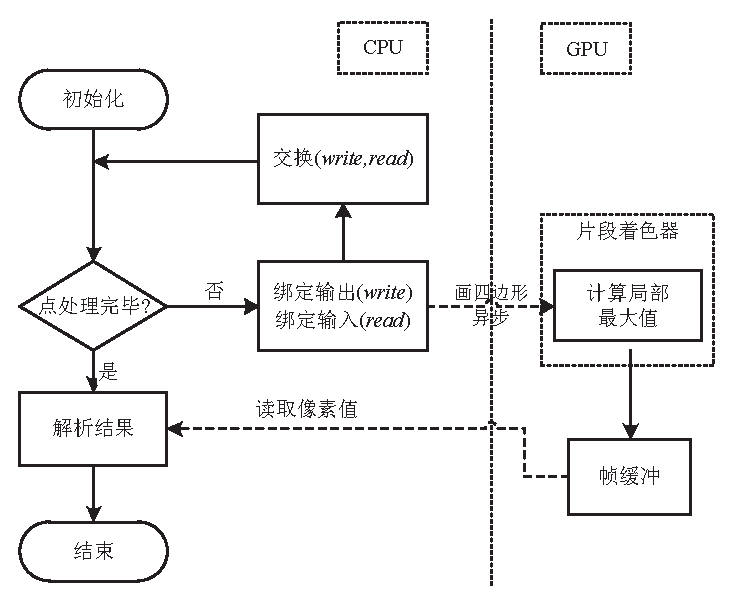
\includegraphics[width=4.2in]{shader-rtt_pp.eps}
  \caption{基于乒乓技术算法流程图}
  \label{fig:shader-rtt-pingpong-flowchart}
\end{figure}

图~\ref{fig:shader-rtt-pingpong-flowchart}~为基于乒乓技术的算法的流程图,算法将所有法向保存在纹理~$read$~中并利用纹理~$write$~缓存中间结果,第~$m$~次渲染进行计算时,纹理~$read$~作为输入,将渲染即计算的结果缓存在纹理~$write$~中,
在第~$m+1$~次渲染时将读取缓存在纹理~$write$~中的数据作为输入,而此时纹理~$read$~又作为输出,如此进行交替,每步交换只更改沿着每个法向的局部最大值。
如代码~\ref{shader:pingpong}~中的片段着色器代码所示,用一个像素值保存法向的~$xyz$~坐标值和沿着该法向投影得到最大值,另外该像素的第四个分量保存该最大值点在输入点数组中的索引。
算法将输入点分成~$x$~份,每次只处理一份,在当前渲染过程中,找出在该批点集中沿着所有法向投影值最大的点,当处理下批点集即下一次渲染时,将与上次局部最大投影值进行比较,若有新的投影最大值就更新,如此反复~$x$~次,
当所有点都被处理完毕后得到沿着所有法向投影最大值的点即切点。最后再通过~CPU~一次性从帧缓冲中读取所有法向的切点。
\lstinputlisting[float=!ht, language={shader}, caption={基于乒乓技术算法着色器代码}, label=shader:pingpong]{shader_rrt_pingpong.frag}

与~Z Buffer~算法相比,基于乒乓技术的算法在进行一次绘制操作能够得到沿着~$k$~个法向的局部(所有处理过的点集)最大值。为了充分利用~GPU~的并行计算能力,将每次处理点的数量设置为~GPU~硬件所支持的~OpenGL~中统一块(uniform
block)所能容纳数据的大小,即需要反复绘制的次数为~$x=n/b$,其中~$n$~为点集大小,$b$~为统一块能容纳点的数量,值与显卡具体型号有关。 

\subsection{基于~CUDA~的并行算法}
\label{subsec:determ-normals-by-cuda}

~CUDA~是显卡公司~NVIDIA~推出的通用的并行计算架构平台,能够利用~GPU~解决并行计算问题,并提供了多种语言的编程接口。
CUDA~程序可以由一系列的主机程序组成,主机程序能够并行地在~GPU~设备上运行,GPU~运算单元将并行的线程分解成线程块,每个线程块又由若干线程组成,GPU~的流水处理器以线程块为单位进行调度。
将问题划分成子问题提交给~GPU~让多线程同时处理这些子问题,这样可以提升算法的效率\cite{lauterbach2009fast}。

如图~\ref{lbl:reduction-getmax}~所示,最大投影值的计算可采用如下规约方式:将输入点交给数量为~$t$~的线程计算点积得到投影值,
线程~$i$~和~$i+t/2$~比较选取较大者,经~$\log_2t$~次比较可得最大值。
这种规约方式也很容易移植到开放计算语言(Open Computing Language,简称~OpenCL)等并行计算框架平台上\cite{gpgpuqiu},在此不再赘述。

\begin{figure}[htbp] % use [htbp] to fix the position
\centering
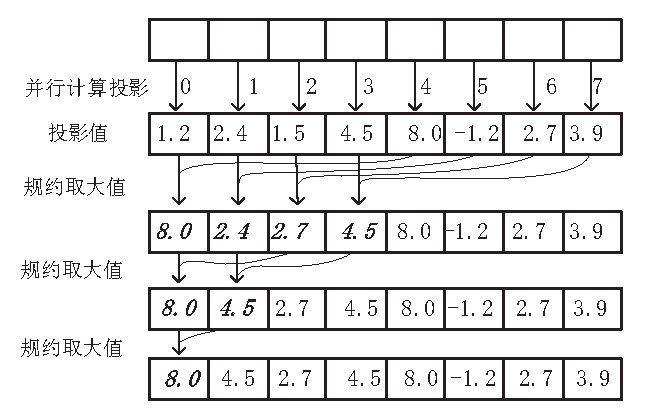
\includegraphics[width=4.2in]{gpureduction.eps}
\caption{并行规约求最大投影值}
\label{lbl:reduction-getmax}
\end{figure}

图~\ref{lbl:reduction-getmax}~所示的示例中,假设有~8~个点与某法向点积得到的投影值为~$(1.2,2.4,1.5,4.5,8.0,-1.2,2.7,3.9)$,有4个线程~同时比较第~$i$~个投影值与~$i+4$~投影值得到新的较大投影值~$(8.0,2.4,2.7,4.5)$,并将新的较大的投影值放入线程~$i$~中,
再以同样的方式规约得到较大的两个投影值~$(8.0,4.5)$,最后再通过一次比较得到最大的投影值~$8.0$~。
文献~\onlinecite{Harris2007Optimizing}介绍了更多更详细规约优化技术。

\section{截面求交算法}
\label{sec:intersect-planes}

确定~$k$-CBP~各个截面后,直接求得所有平面的交点并排除在平面外部的交点即可得到~$k$-CBP~的顶点。该问题即转化为:给定~$k$~个平面及其法向,平面及法向相当于一个半空间~$\bm{H}$,即已知集合$\{\bm{H_1},
\bm{H_2}, \cdots, \bm{H_k}\}$,求$\bm{H_1} \cap \bm{H_2} \cap \cdots
\cap \bm{H_k}$。该问题是一个线性规划(Linear Programming)问题,文献~\onlinecite{dengcg}~详细介绍了在二维线性规划下的相关算法,本文将分别介绍一种直观的枚举算法和利用对偶映射的方法求得~$k$-CBP~的交点。

\subsection{枚举法}
\label{subsec:intersection-enum-geometry}

空间中的平面位置情况如图~\ref{fig:three-planes-intersection}~所示,可分为如下几种情况:
\begin{inparaenum}[(1)]
\item \textbf{无交点},若3个平面互相平行则没有交点,如图~\ref{lbl:intersection-center-0}~所示;
\item \textbf{1~条交线}, 如图~\ref{lbl:intersection-center-1}~所示,3个平面相交于~1~条交线;
\item \textbf{2~条交线}, 当有两个平面互相平行,另一个平面与其相交时有2条交线,如图~\ref{lbl:intersection-center-2}~;
\item \textbf{3~条交线}, 如图~\ref{lbl:intersection-center-3}~所示,3个平面交于~3~条交线;
\item \textbf{1~个交点}, 最后一种情况是三个平面相交于1点的情况,如图~\ref{lbl:intersection-center-4}~所示。
\end{inparaenum}

一个凸多面体的每一个顶点都可看作是至少3个平面的交点。现在只需要枚举出所有3个平面相交于1点的所有情况即可得到$k$-CBP~的顶点,值得注意的是,并非所有交点都是多面体的顶点,交点在某个半空间的正方向上即在半空间相交区域的外部须排除。

\begin{figure}[htbp]
  \centering
  \subcaptionbox{没有交点\label{lbl:intersection-center-0}}{%
    
\includegraphics[width=1.8in]{intersection-center-0.png}}\hspace{1em}%
  \subcaptionbox{交于~1~条线\label{lbl:intersection-center-1}}{%
    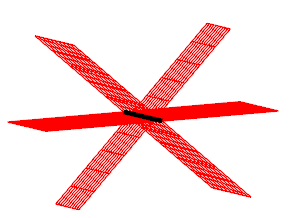
\includegraphics[width=1.8in]{intersection-center-1.png}}\hspace{1em}%
  \subcaptionbox{交于~2~条线\label{lbl:intersection-center-2}}{%
    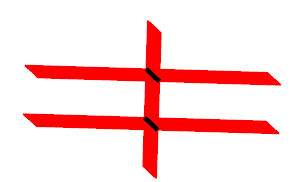
\includegraphics[width=1.8in]{intersection-center-2.png}}%
  \\
  \subcaptionbox{交于~3~条线\label{lbl:intersection-center-3}}{%
    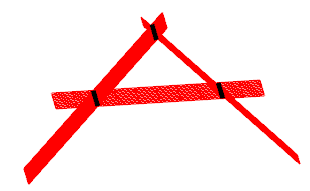
\includegraphics[width=2.3in]{intersection-center-3.png}}%
  \subcaptionbox{交于~1~个点\label{lbl:intersection-center-4}}{%
    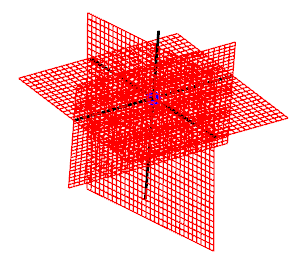
\includegraphics[width=2.0in]{intersection-center-4.png}}%
  \caption{空间中~3~个平面的相交情况}
  \label{fig:three-planes-intersection}
\end{figure}

假设满足如图~\ref{lbl:intersection-center-4}~所示的三个平面的法向分别是$\bm{n_1}, \bm{n_2}, \bm{n_3}$,
平面上一点分别为~$\bm{p_1}, \bm{p_2}, \bm{p_3}$,则三个平面的交点须满足如下方程: 
\begin{equation}
  \label{equa:three-planes-intersection}
  \left\{
    \begin{array}{l}
      \bm{n_1} \cdot \bm{x} = \bm{n_1} \cdot \bm{p_1}\\
      \bm{n_2} \cdot \bm{x} = \bm{n_2} \cdot \bm{p_2}\\
      \bm{n_3} \cdot \bm{x} = \bm{n_3} \cdot \bm{p_3}
    \end{array}
    \right.
\end{equation}

令$(\bm{n_1} \cdot \bm{p_1}, \bm{n_2} \cdot \bm{p_2}, \bm{n_3} \cdot \bm{p_3})
= (y_1, y_2, y_3) = \bm{y}$,则求解式(\ref{equa:three-planes-intersection})相当于解线性方程组
$\bm{A} \bm{x}=\bm{y}$ 即 $(\bm{n_1},\bm{n_2}, \bm{n_3})^T \cdot \bm{x} = \bm{y}$, 令
$\bm{n_i} = (a_{i1}, a_{i2}, a_{i3}), i=\{1,2,3\}$,则有:
\begin{equation*}
  \label{equa:matrix:crammer}
  \left(
    \begin{array}{ccc}
      a_{11} & a_{12} & a_{13} \\
      a_{21} & a_{22} & a_{23} \\
      a_{31} & a_{32} & a_{33} \\
    \end{array}
  \right)
  \cdot 
  \bm{x} 
 % \left(
 %   \begin{array}{c}
 %     x_{1} \\
 %     x_{2} \\
 %     x_{3} \\
 %   \end{array}
 % \right)
  =
  \left(
    \begin{array}{c}
      y_{1} \\
      y_{2} \\
      y_{3} \\
    \end{array}
  \right)
\end{equation*}

根据克莱姆法则(Crammer's Rule),上述方程有唯一解,则
$|\bm{A}| \not= 0$,且解~$x_i = \frac{|\bm{A_i}|}{|\bm{A}|}, i =
\{1,2,3\}$,其中~$|\bm{A}_i|$~是矩阵~$\bm{A}$~中将第~$i$~列替换成~$\bm{y}^T$~之后的行列式,在计算~$\bm{A}_i$~和~$|\bm{A}|$~时为了避免一些重复计算,将其展开有:
\begin{equation*}
 \left\{
\begin{array}{llll}
%\begin{aligned}
    |\bm{A}|   &=
    a_{11}  \left|
                  \begin{array}{cc}
                    a_{22} & a_{23} \\
                    a_{32} & a_{33} \\
                  \end{array}
              \right|
    &- a_{12} \left|
                  \begin{array}{cc}
                    a_{21} & a_{23} \\
                    a_{31} & a_{33} \\
                  \end{array}
              \right|
    &+ a_{13}
              \left|
                  \begin{array}{cc}
                    a_{21} & a_{22} \\
                    a_{31} & a_{32} \\
                  \end{array}
              \right|
\vspace{0.5em}\\ \vspace{0.5em}
    |\bm{A}_1| &= 
    y_1     \left|
                  \begin{array}{cc}
                    a_{22} & a_{23} \\
                    a_{32} & a_{33} \\
                  \end{array}
              \right|
    &- a_{12} \left|
                  \begin{array}{cc}
                    y_2 & a_{23} \\
                    y_3 & a_{33} \\
                  \end{array}
              \right|
    &+ a_{13}
              \left|
                  \begin{array}{cc}
                    y_2 & a_{22} \\
                    y_3 & a_{32} \\
                  \end{array}
              \right|
\\ \vspace{0.5em}
    |\bm{A}_2| &= 
    a_{11}  \left|
                  \begin{array}{cc}
                    y_{2} & a_{23} \\
                   y_{3} & a_{33} \\
                  \end{array}
              \right|
    &- y_{1}  \left|
                  \begin{array}{cc}
                    a_{21} & a_{23} \\
                    a_{31} & a_{33} \\
                  \end{array}
              \right|
    &+ a_{13}
              \left|
                  \begin{array}{cc}
                    a_{21} & y_{2} \\
                    a_{31} & y_{3} \\
                  \end{array}
              \right|
\\ \vspace{0.5em}
    |\bm{A}_3| &= 
    a_{11}  \left|
                  \begin{array}{cc}
                    a_{22} & y_{2} \\
                    a_{32} & y_{3} \\
                  \end{array}
              \right|
    &- a_{12} \left|
                  \begin{array}{cc}
                    a_{21} & y_{2} \\
                    a_{31} & y_{3} \\
                  \end{array}
              \right|
    &+ y_{1}
              \left|
                  \begin{array}{cc}
                    a_{21} & a_{22} \\
                    a_{31} & a_{32} \\
                  \end{array}
              \right|
\end{array}
%\end{aligned}
\right.
\end{equation*}

%TODO 下面可用一个大括号括起来
令
%$b_1 = \left|
%\begin{array}{cc}
%  a_{22} & a_{23} \\
%  a_{32} & a_{33} 
%\end{array} 
%\right|
%  = a_{22}a_{33} - a_{32}a_{23}
%,
%b_2 = \left|
%\begin{array}{cc}
%  a_{21} & a_{23} \\
%  a_{31} & a_{33} 
%\end{array} 
%\right|
%  = a_{21}a_{33} - a_{31}a_{23}
%,
%b_3 = \left|
%\begin{array}{cc}
%  a_{21} & a_{22} \\
%  a_{31} & a_{32} \\
%\end{array}
%\right|
%= a_{21}a_{32}-a_{31}a_{22}
%,
%b_4 = \left|
%  \begin{array}{cc}
%    y_2 & a_{23} \\
%    y_3 & a_{33} \\
%  \end{array}
%\right|
%  = y_2a_{33}-y_3a_{23}
%,
%b_5 = \left|
%  \begin{array}{cc}
%      y_2 & a_{22} \\
%      y_3 & a_{32} \\
%      \end{array}
%    \right|
%  = y_2a_{32}-y_3a_{22}
%,
%b_6 = \left|
%    \begin{array}{cc}
%      a_{21} & y_{2} \\
%      a_{31} & y_{3} \\
%    \end{array}
%  \right|
%  =a_{21}y_{3}-a_{31}y_{2}
%$
\begin{equation*}
  \left\{
    \begin{array}{lll}
        b_1 &= \left|
        \begin{array}{cc}
          a_{22} & a_{23} \\
          a_{32} & a_{33} 
        \end{array} 
        \right|
         &= a_{22}a_{33} - a_{32}a_{23}
        \\
        b_2 &= \left|
        \begin{array}{cc}
          a_{21} & a_{23} \\
          a_{31} & a_{33} 
        \end{array} 
        \right|
          &= a_{21}a_{33} - a_{31}a_{23}
        \\
        b_3 &= \left|
        \begin{array}{cc}
          a_{21} & a_{22} \\
          a_{31} & a_{32} \\
        \end{array}
        \right|
        &= a_{21}a_{32}-a_{31}a_{22}
        \\
        b_4 &= \left|
          \begin{array}{cc}
            y_2 & a_{23} \\
            y_3 & a_{33} \\
          \end{array}
        \right|
         & = y_2a_{33}-y_3a_{23}
        \\
        b_5 &= \left|
          \begin{array}{cc}
              y_2 & a_{22} \\
              y_3 & a_{32} \\
              \end{array}
            \right|
          &= y_2a_{32}-y_3a_{22}
        \\
        b_6 &= \left|
            \begin{array}{cc}
              a_{21} & y_{2} \\
              a_{31} & y_{3} \\
            \end{array}
          \right|
          &=a_{21}y_{3}-a_{31}y_{2}
    \end{array}
\right.
\end{equation*}
则有:
\begin{equation}
  \label{equa:solution:three-planes}
  \left\{
    \begin{array}{lll}
      x_1 =& \frac{|\bm{A_1}|}{|\bm{A}|} =&\frac{y_1b_1-a_{12}b_4+a_{13}b_5}{a_{11}b_1-a_{12}b_2+a_{13}b_3} 
      \vspace{0.5em}\\ \vspace{0.5em}
      x_2 =& \frac{|\bm{A_2}|}{|\bm{A}|} =&\frac{a_{11}b_4-y_{1}b_2+a_{13}b_6}{a_{11}b_1-a_{12}b_2+a_{13}b_3} 
      \\ \vspace{0.5em}
      x_3 =& \frac{|\bm{A_3}|}{|\bm{A}|} =&\frac{-a_{11}b_5-a_{12}b_6+y_{1}b_3}{a_{11}b_1-a_{12}b_2+a_{13}b_3}
    \end{array}
  \right.
\end{equation}其中,$|\bm{A}| \not= 0$。


\begin{algorithm}[htbp]
\small
\caption{截面求交枚举算法}
\label{alg:enum_algortihm}
\begin{algorithmic}[1]
\Require
平面~$planes$
\Ensure
凸包围多面体~$k$-CBP
\Function{ConstructKCBP}{$planes$}
  \ForAll {$p_1 \in planes$}
    \State $Intersection \gets \emptyset $
    \ForAll {$p_2 \in planes$}
          \ForAll {$p_3 \in planes$}
              %\If{$ (p_1 = p_2 || p_1 = p_3 || p_2 = p_3) = \FALSE $}
              \If{$ p_1 \nparallel p_2 \nparallel p_3$}
                  \If{$|A| \not= 0$}
                      \State $P = \Call{vec3}{x_1, x_2, x_3}$
                      \Comment{按照公式(\ref{equa:solution:three-planes})计算得到交点坐标值} 
                      \If{\Call{validate}{P}}
                        \State \Comment{验证交点P是否都在半空间负方向上}
                        \State $Intersection \gets Intersection \cup P$
                      \EndIf
                  \EndIf
              \EndIf
          \EndFor
     \EndFor
     \If {$Intersection.size \geq 3$}
     \State {$k\textrm{-CBP} \gets k\textrm{-CBP} \cup \Call{polygon}{p_1, Intersection}$}
     \Comment{满足条件,加入到结果集}
     \EndIf
  \EndFor
  \State \Return {$k$-CBP}
\EndFunction
\end{algorithmic}
\end{algorithm}

完整的算法如算法~\ref{alg:enum_algortihm}~所示,算法输入为第~\ref{sec:search:planes}节中得到的截面$planes$,输出为~$k$-CBP~,每个~$k$-CBP~的多边形截面由围成多边形的交点和多边形所在平面构成。
算法枚举遍历所有平面的组合,搜索出三个平面交于一点的情况,排除在半空间外部的交点即可得到~$k$-CBP~的顶点,算法复杂度为~$O(k^3)$,此算法思想简单易于理解和实现,但当平面数量较多(即~$k$~值较大)时,会耗费很多时间,与枚举法相比基于对偶映射的算法实现较复杂但其时间复杂度为~$O(k \log k)$,效率更高。

\subsection{对偶映射算法}
\label{subsec:intersection-dual-mapping}

正如~$k$-CBP~的定义所知,$k$-CBP~可看作是多个半空间的交集,一个半空间可由法向$\bm{n}(a,b,c)$及离原点距离~$d$~确定,转换为线性不等式即为
\begin{equation}
  \label{equa:halfspace:defition}
  a_ix+b_iy+c_iz \leq d_i, \quad i=1,2,\cdots,k,
\end{equation}
其中~$a_i,b_i,c_i,d_i$~是不同时为0的实数。

求解~$k$-CBP~可将问题转换为求~$k$~个线性不等式的解。利用对偶映射的方式可在~$O(k \log k)$~的方式解决,
具体方法分为三个步骤\cite{Preparata1985Introduction}:
\\ \indent
\begin{inparaenum}[(1)]
%\begin{enumerate}[(1)]
\item   
首先,将上述线性不等式对偶映射成一个欧式空间上的三维点,
$a_ix+b_iy+c_iz=d_i \rightarrow \bm{p}(-a_i/d_i, -b_i/d_i,-c_i/d_i),d_i \neq 0$,其中~$(a_i,b_i,c_i)$~为第~\ref{sec:search:planes}~节中得到的
截面法向~$\bm{n}$,$d_i=\bm{n} \cdot
max\_point$~为截面法向与截面上的投影点~$max\_point$~的点积,此步骤的算法复杂度为~$O(k)$; \\ \indent
\item
其次,对对偶映射得到的欧式空间~$k$~个点求凸包,此步骤的算法复杂度为~$O(k\log k)$~,可用第~\ref{subsec:convexhull}~节中的分治算法; \\ \indent
\item
  得到凸包后,再利用相同的对偶变换将凸包平面方程映射回欧式空间三维点,这些点即为原始半空间的交点,此步骤的算法复杂度仍为~$O(k)$。
\end{inparaenum}
%\end{enumerate}

综上,该方法总体复杂度为~$O(k\log k)$~。
在利用这种对偶变化时需要注意约束条件即上述不等式中的~$d_i>0$,此时原点~$O(0,0,0)$~始终满足不等式(\ref{equa:halfspace:defition}),体现在算法输入上即原始模型需要包含原点。当原始模型不包含原点时,可以先对模型做一定平移或者也可用另外的对偶变换进行求解,文献\onlinecite{Preparata1979Intersection}对此问题进行了详述的阐述。

\section{实验结果及分析}
\label{sec:exper-kcbp}

本文将针对不同点集规模的模型进行测试\footnote{运行时环境为:Intel(R) Core(TM)
i5-2320 CPU @ 3.2GHz 8G RAM NVIDIA GeForce GTX
650。},从两个角度对生成的~$k$-CBP~进行实验对比,
一方面对生成~$k$-CBP~的速度进行效率上的对比,主要对比了串行算法、基于着色器和~CUDA~环境的并行算法和文献\onlinecite{karlsson2010parallel}的并行算法,其详细结果如~\ref{subsec:exper:efficiency}~节所示;
另一个方面对生成~$k$-CBP~的质量即紧致性上进行了对比实验,主要围绕着凸包、文献\onlinecite{abenchmarking2007}~中实现的~$k$-DOP~进行对比,详细结果见第~\ref{subsec:exper:tightness}~节。

\subsection{凸包围多面体生成效率}
\label{subsec:exper:efficiency}

如图~\ref{fig:chart:exps:cputime}~所示为本文算法(CUDA)与传统的~CPU~算法对比结果,图中横纵坐标分别代表多面体面数和运行时间,其中实线~CPU$\rm{'}$~和$k$-CBP$\rm{'}$分别表示用传统~CPU~方法和本文~CUDA~算法构造凸包围多面体总体耗时,虚线~CPU~和$k$-CBP~分别代表各自算法搜索截面的过程。
从中可以看出,当模型点数量较大时,搜索截面的过程占据了算法绝大多数时间,且随着凸包围多面体的面数~$k$~值增加而线性增长,这与搜索截面时间复杂度~$O(k\cdot
n)$一致,截面求交过程利用第~\ref{subsec:intersection-dual-mapping}~节中的对偶映射法,其时间复杂度为~$O(k\log k)$,
当点数量极大时,如图~\ref{fig:exp:cpu:buggatti}~所示,实线虚线几乎重合即求交等步骤耗时相比整体算法而言几乎可忽略。
当输入模型的点数量越大,本文算法的优势越明显。如~Budda~模型点数量~31k~左右,加速比约为~3 $\sim$ 6~倍,而含有~224k~个点的~Alice~模型和~1010k~个点的~Bugatti~模型,能够加速~7$\sim$9~倍。

\begin{figure}[!ht] % use [htbp] to fix the position
\centering
\subcaptionbox{Budda模型(31232个点)\label{fig:exp:cpu:budda}}
{  
   \includegraphics[width=\fourgraphicswidth\textwidth,page=2]{cudatime.pdf}
}
\subcaptionbox{Dinosaur模型(40277个点)\label{fig:exp:cpu:Dinasour}}
{  
    \includegraphics[width=\fourgraphicswidth\textwidth, page=3]{cudatime.pdf}
}\linebreak %强制换行
\subcaptionbox{Alice模型(224291个点)\label{fig:exp:cpu:alice}}
{  
   \includegraphics[width=\fourgraphicswidth\textwidth, page=4]{cudatime.pdf}
}
\subcaptionbox{Bugatti模型(1010815个点)\label{fig:exp:cpu:buggatti}}
{  
   \includegraphics[width=\fourgraphicswidth\textwidth, page=5]{cudatime.pdf}
}
\caption{基于~CUDA~并行算法运行时间}
\label{fig:chart:exps:cputime}
\end{figure}

图~\ref{fig:chart:exps:shadertime}~为着色器算法根据不同模型构造不同面数的包围体所耗费的时间对比,横坐标表示多面体面数~$k$,纵坐标为运行时间,曲线~cpu、zbuffer和rtt\_pp分别表示基于CPU、深度缓冲(Z Buffer)和基于乒乓技术的算法的运行时间。

\begin{figure}[!ht] % use [htbp] to fix the position
\centering
\subcaptionbox{Apple模型(8118个点)\label{fig:exp:shader:apple}}
{  
   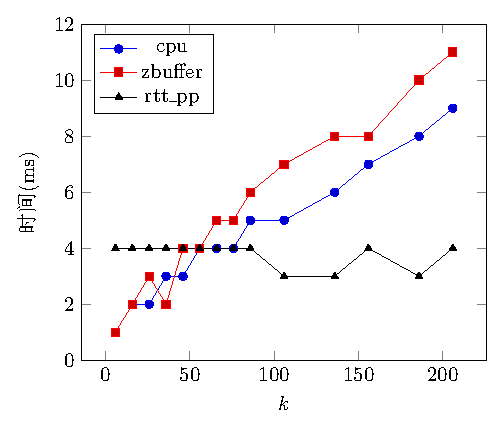
\includegraphics[width=\fourgraphicswidth\textwidth,page=1]{shadertime.pdf}
}
\subcaptionbox{Buddha模型(31232个点)\label{fig:exp:shader:buddha}}
{  
    \includegraphics[width=\fourgraphicswidth\textwidth, page=2]{shadertime.pdf}
}\linebreak %强制换行
\subcaptionbox{Alice模型(224291个点)\label{fig:exp:shader:alice}}
{  
   \includegraphics[width=\fourgraphicswidth\textwidth, page=3]{shadertime.pdf}
}
\subcaptionbox{Bugatti模型(1010815个点)\label{fig:exp:shader:buggatti}}
{  
   \includegraphics[width=\fourgraphicswidth\textwidth, page=4]{shadertime.pdf}
}
\caption{基于着色器的并行算法运行时间}
\label{fig:chart:exps:shadertime}
\end{figure}

从实验结果可以看出,当模型规模不大时,如图~\ref{fig:exp:shader:apple}~所示的含有8千多个点的~Apple~模型,
Z Buffer~算法和传统的~CPU~算法差别不是很大,因此在实际应用中当模型规模较小时可直接用~CPU~计算即可。
随着输入模型所含有点的数量规模的增加,CPU~和~GPU~运行时间之间的差距也越来越大。
当多面体面数增加即~$k$~的增大时,在~Z Buffer~算法中,需要更多的绘制次数,因此其运行时间也有所增加,而在基于乒乓技术的算法中,当点规模一定时,$k$~的变化对最后运行时间影响不明显,因此当较大的~$k$~时,这种算法更快。

\begin{table}[htbp]
\centering
\caption{基于着色器并行算法加速比}
\label{tab:exper:shadertime}
\begin{minipage}[c]{\textwidth}
\begin{center}
  \begin{tabular}{p{1.5cm}<{\centering}cccc cccc} %p本身占一列
  \toprule[1.5pt]
  \multirow{3}{*}{$k$} & \multicolumn{4}{c}{Apple模型(8118 个点)} & \multicolumn{4}{c}{Bugatti~模型(1010815个点)}\\
  \cmidrule(lr){2-5}\cmidrule(lr){6-9}
  & cpu & zbuffer  & rtt\_pp & \multirow{2}{*}{加速比$^{(a)}$} & cpu  & zbuffer& rtt\_pp & \multirow{2}{*}{加速比$^{(a)}$} \\
  & (ms) & (ms)  & (ms) & & (ms)  & (ms) & (ms) \\
  \midrule[1pt]
 6	 & 6 	& 5 	& 41 &	1.20 &	26	& 17	&178  &	1.53 \\
16	 & 16	& 13	& 43 &	1.23 &	70	& 48	&181  &	1.46 \\
26	 & 25	& 17	& 43 &	1.47 &	114	& 68	&183  &	1.68 \\
36	 & 34	& 17	& 45 &	2.00 &	153	& 70	&178  &	2.19 \\
46	 & 44	& 24	& 42 &	1.83 &	203	& 102	&176  &	1.99 \\
56	 & 53	& 31	& 43 &	1.71 &	241	& 131	&177  &	1.84 \\
66	 & 62	& 39	& 43 &	1.59 &	285	& 162	&179  &	1.76 \\
76	 & 73	& 46	& 46 &	1.59 &	331	& 196	&189  &	1.75 \\
86	 & 82	& 52	& 45 &	1.82 &	373	& 225	&192  &	1.94 \\
106	 & 100	& 59	& 45 &	2.22 &	464	& 257	&191  &	2.43 \\
136	 & 127	& 81	& 42 &	3.02 &	604	& 349	&180  &	3.36 \\
156	 & 146	& 88	& 47 &	3.11 &	693	& 378	&202  &	3.43 \\
186	 & 177	& 110	& 43 &	4.12 &	861	& 474	&180  &	4.78 \\
206	 & 194	& 123	& 49 &	3.96 &	962	& 533	&209  &	4.60 \\
  \bottomrule[1.5pt]
\end{tabular}
\end{center}\vspace{-0.5em}
\hspace{1em}
\footnotesize (a): 加速比=~cpu/$min$(zbuffer, rtt\_pp)
\end{minipage}
\end{table}

表~\ref{tab:exper:shadertime}~详细的展示了基于着色器的两种算法应用于~Alice~和~Bugatti~模型的构造时间及相应的加速比。
从中可看出,Z Buffer~算法适合相对较小的~$k$~值,而基于乒乓技术的算法在较大~$k$~值时能达到更大的加速比。

本文实现了文献~\onlinecite{karlsson2010parallel}~中的并行算法并进行对比实验,表~\ref{tab:exp:sse-time}
~为实验统计结果,表中数据均为搜索截面耗时,因为二者其他步骤均相同且从~\ref{fig:chart:exps:cputime}~可得搜索截面时间占用整体绝大部分时间,其中~$k$~为多面体面数,
列~SSE~和列~$k$-CBP~分别为文献~\onlinecite{karlsson2010parallel}~中的算法和本文提出的基于~CUDA~算法的运行时间。

\begin{table}[htbp] 
\centering
\caption{本文算法与文献~\onlinecite{karlsson2010parallel}~的并行算法对比}
\begin{tabular}{p{1.5cm}<{\centering}ccc ccc} %p本身占一列
\toprule[1.5pt]
\multirow{2}{*}{$k$} & \multicolumn{3}{c}{Apple模型(8118个点)} &
\multicolumn{3}{c}{Bugatti~模型(1010815个点)}\\
\cmidrule(lr){2-4}\cmidrule(lr){5-7}
~&SSE\cite{karlsson2010parallel}(ms) & $k$-CBP(ms) &  加速比 & SSE\cite{karlsson2010parallel}(ms) & $k$-CBP(ms) &  加速比\\
\midrule[1pt]
6 & 0.4 & 0.12  & 3.20     & 24.2 & 3.20  & 7.56 \\
16 & 0.9 & 0.26  & 3.43    & 44.5 & 8.44  & 5.27 \\
26 & 1.4 & 0.41  & 3.38    & 66.5 & 13.65  & 4.87 \\
36 & 1.9 & 0.52  & 3.65    & 91.1 & 18.34  & 4.97 \\
46 & 2.5 & 0.67  & 3.74    & 119.5 & 24.13  & 4.95 \\
56 & 2.9 & 0.79  & 3.66    & 138.4 & 28.86  & 4.80 \\
66 & 3.5 & 0.95  & 3.69    & 170.6 & 34.10  & 5.00 \\
76 & 4.0 & 1.08  & 3.70    & 197.1 & 39.85  & 4.95 \\
86 & 4.5 & 1.22  & 3.69    & 219.8 & 45.08  & 4.88 \\
106 & 5.4 & 1.49  & 3.62   & 267.8 & 55.52  & 4.82 \\
136 &  6.8 & 1.92  & 3.54  & 342.9 & 71.24  & 4.81 \\
156 &  7.7 & 2.17  & 3.55  & 411.3 & 81.18  & 5.07 \\
186 &  9.3 & 2.60  & 3.58  & 479.4 & 97.39  & 4.92 \\
206 &  10.5 & 2.85  & 3.68 & 523.0 & 106.87  & 4.89  \\  
\bottomrule[1.5pt]
\end{tabular}
\label{tab:exp:sse-time}
\end{table}

与文献~\onlinecite{karlsson2010parallel}~中的算法相比,本文算法优势明显。
当用于点数量较小~Apple~模型时,能够提高~3$\sim$4~倍速度,模型变大,加速比也更大,~Bugatti~模型的提速达到~4$\sim$8~倍。

\subsection{凸包围多面体紧致程度}
\label{subsec:exper:tightness}

凸包围多面体的质量用公式(\ref{equa:judge:tightness})衡量即通过凸包与凸包围多面体的体积之比来量化包围体的紧致程度。
文献~\onlinecite{abenchmarking2007}~是基于~$k$-DOP~实现的层次结构的包围体,其顶层的~$k$-DOP~与本文算法生成的~$k$-CBP~的紧致程度对比如图~\ref{chart:exps:tightness}~所示,
图中横坐标~$k$~为凸包围多面体的面数,纵坐标为紧致程度,曲线~$k$-DOP~和~$k$-CBP~分别为文献~\onlinecite{abenchmarking2007}~和本文的方法,由图可知,
对于不同模型,本文构造的凸包围多面体紧致程度均有所提升,如~Alice~模型提升了12.08\%,~Dinasour~模型提升了34.0\%。
以~$k \in \{20,38\}$~为例,相应模型的~$k$-DOP~和~$k$-CBP~效果可见图~\ref{fig:kdop:kcbp:ui}。

\begin{figure}[htbp] 
\centering
\subcaptionbox{Apple(8118个点)\label{fix:exp:tightness:apple}}
{
    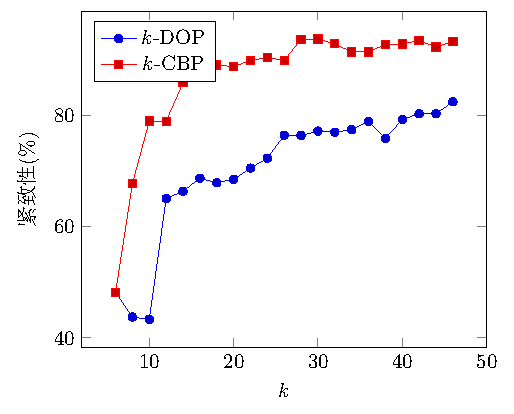
\includegraphics[width=\fourgraphicswidth\textwidth,page=1]{tightness.pdf}
}
\subcaptionbox{Budda(31232个点)\label{fix:exp:tightness:budda}}
{  
   \includegraphics[width=\fourgraphicswidth\textwidth,page=2]{tightness.pdf}
}
\linebreak
\subcaptionbox{Dinosaur(40277个点)\label{fix:exp:tightness:Dinasour}}
{  
    \includegraphics[width=\fourgraphicswidth\textwidth, page=3]{tightness.pdf}
}
\subcaptionbox{Alice(224291个点)\label{fix:exp:tightness:alice}}
{  
   \includegraphics[width=\fourgraphicswidth\textwidth, page=4]{tightness.pdf}
}
\caption{紧致程度对比:$k$-DOP~为文献~\onlinecite{abenchmarking2007}~的算法, $k$-CBP~为本文算法}
\label{chart:exps:tightness}
\end{figure}

\begin{figure}[htbp] 
\centering
\subcaptionbox{Bunny(20-DOP和20-CBP)}
{  
   \includegraphics[width=0.40\linewidth]{bunny-kcbp-dop-20.png}
 }
\subcaptionbox{Bunny(38-DOP和38-CBP)}
{
    \includegraphics[width=0.40\linewidth]{bunny-kcbp-dop-38.png}
}
\linebreak
\subcaptionbox{Apple(20-DOP和20-CBP)}
{  
   \includegraphics[width=0.45\linewidth]{apple-kcbp-dop-20.png}
}
\subcaptionbox{Apple(38-DOP和38-CBP)}
{  
   \includegraphics[width=0.45\linewidth]{apple-kcbp-dop-38.png}
}
\linebreak
\subcaptionbox{Budda(20-DOP和20-CBP)}
{  
   \includegraphics[width=0.40\linewidth]{budda-kcbp-dop-20.png}
 }\hspace{1.5em}
\subcaptionbox{Budda(38-DOP和38-CBP)}
{
    \includegraphics[width=0.40\linewidth]{budda-kcbp-dop-38.png}
}
\linebreak
\subcaptionbox{Dinosaur(20-DOP和20-CBP)}
{  
   \includegraphics[width=0.48\linewidth, height=0.16\linewidth]{dinosaur-kcbp-dop-20.old.eps}
}
\subcaptionbox{Dinosaur(38-DOP和38-CBP)}
{  
   \includegraphics[width=0.48\linewidth, height=0.16\linewidth]{dinosaur-kcbp-dop-38.old.eps}
}
\linebreak
\subcaptionbox{Alice(20-DOP和20-CBP)}
{  
   \includegraphics[width=0.38\linewidth]{alice-kcbp-dop-20.png}
 }\hspace{1.5em}
\subcaptionbox{Alice(38-DOP和38-CBP)}
{
    \includegraphics[width=0.38\linewidth]{alice-kcbp-dop-38.png}
}
\caption{~$k$-CBP~与~$k$-DOP~对比}
\label{fig:kdop:kcbp:ui}
\end{figure}

\begin{table}[htbp]   
\centering
\caption{用近似凸包与精确凸包构造~$k$-CBP~紧致程度对比}
\label{tab:exp:ach:ch:tightness}
\begin{tabular}{lccccl}
\toprule[1.5pt]
$k$ &  $\tau$(ACHull)(\%) & $\tau$ (CHull)(\%)  & $k$ &  $\tau$ (ACHull)(\%) & $\tau$ (CHull)(\%) \\
\midrule[1.0pt]
10 &	70.44 & 	65.56     &26 &	89.93 & 	94.45 \\
12 &	74.56 & 	75.63     &28 &	88.61 & 	92.24 \\
14 &	79.50 & 	82.49     &30 &	91.58 & 	92.35 \\
16 &	84.79 & 	85.20     &32 &	92.78 & 	93.78 \\
18 &	85.75 & 	90.09     &34 &	91.28 & 	93.22 \\
20 &	86.38 & 	90.36     &36 &	92.93 & 	94.68 \\
22 &	90.27 & 	92.48     &38 &	93.41 & 	93.20 \\
24 &	90.70 & 	93.09     &40 &	93.81 & 	94.70 \\
\bottomrule[1.5pt]
\end{tabular}
\end{table}

本文算法利用近似凸包与精确凸包的相似性,从近似凸包的众多面片对应的法向中通过~$k$-means~聚类算法生成~$k$~个法向。
表~\ref{tab:exp:ach:ch:tightness}~为利用~Alice~模型的近似凸包和精确凸包分别聚类生成法向构造~$k$-CBP~的紧致程度对比。
可以看出,一方面,利用精确凸包构造的~$k$-CBP~并不一定比近似凸包构造的结果更紧致,但由于近似凸包与精确凸包的外观的近似性因此二者得到的结果相差并不大(5\%以内);
另一方面,因近似凸包的时间复杂度为线性,而精确凸包为~$O(n\log n)$,
因此本文利用近似凸包聚类生成法向。示例中构造近似凸包耗费时间仅为~0.88ms~,而精确凸包为~79.31ms~。


\begin{table}[htbp] 
\centering
\caption{$k$-CBP~与~QuickHull~凸包算法比较}
\label{tab:exp:cgal}
\begin{tabular}{lcccccl}
\toprule[1.5pt]
 Model & $f$(CHull)& $f$($k$-CBP) & $\tau$ ($k$-CBP)(\%) & $t$(CHull)(ms) & $t$($k$-CBP)(ms)\\ % 后面重新跑的, KCBP加上了近似凸包及求交时间的总和, 和近似凸包的分组时间也加了.
\midrule[1.0pt]
  Apple	& 499 & 30 & 93.67 & 5.5 & 1.30 \\ % apple3  自己电脑跑的数据, 之前是用的chengxianyu的电脑.
  Budda	& 1608 & 46 & 92.39 & 21.3 & 2.86 \\ %  1.0+0.86+1
  Dinosaur	& 1240 & 44 & 93.34 & 22.6 & 1.99 \\  % 1.0+0.98+0.1
  Alice	& 1332 & 44 & 93.92 & 85.8 & 8.47\\ % 2+6.48
  Bugatti & 24654 & 44 & 95.06 & 688.7 & 25.41 \\
\bottomrule[1.5pt]
\end{tabular}
\end{table}

\begin{figure}[!ht] 
\centering
\subcaptionbox{Alice(44-CBP)\label{fig:exp:alice}}
{  
   \includegraphics[width=0.20\textwidth]{alice-44-w-n.png}
}
\subcaptionbox{Apple(30-KCBP)\label{fig:exp:apple}}
{
    \includegraphics[width=0.28\textwidth]{apple-30-w-n.png}
}
\subcaptionbox{Bugatti(44-CBP)\label{fig:exp:buggati}}
{  
  \rotatebox{-80}{\includegraphics[width=0.32\textwidth]{buggati-44-w-n.png}}
}
\subcaptionbox{Budda(46-CBP)\label{fig:exp:budda}}
{  
   \includegraphics[width=0.20\textwidth]{budda-46-w-n.png}
}
\linebreak
\subcaptionbox{Alice(CHull)\label{fig:exp:ch:alice}}
{  
   \includegraphics[width=0.20\textwidth]{alice-convexhull.png}
}
\subcaptionbox{Apple(CHull)\label{fig:exp:ch:apple}}
{
    \includegraphics[width=0.28\textwidth]{apple-convexhull.png}
}
\subcaptionbox{Bugatti(CHull)\label{fig:exp:ch:buggati}}
{  
  \rotatebox{-80}{\includegraphics[width=0.32\textwidth]{bugatti-convexhull.png}}
}
\subcaptionbox{Budda(CHull)\label{fig:exp:ch:budda}}
{  
   \includegraphics[width=0.20\textwidth]{budda-convexhull.png}
}
\linebreak
\subcaptionbox{Dinasour(44-CBP)\label{fig:exp:dinosaur}}
{
    \rotatebox{0}{\includegraphics[width=0.38\textwidth]{dinosaur-44-w-n.png}}
}
\subcaptionbox{Dinosaur(CHull)\label{fig:exp:ch:dinosaur}}
{  
    \rotatebox{0}{\includegraphics[width=0.40\textwidth]{dinosaur-convexhull.png}}
}
\caption{~$k$-CBP~与凸包对比}
\label{pic:exps:ch-kcbp}
\end{figure}


本文算法与~CGAL~库中利用~QuickHull~算法构造的凸包进行比较的结果如表~\ref{tab:exp:cgal}~所示,
其中~$f$(CHull)~和~$f$($k$-CBP)~分别表示凸包的面数和凸包围多面体的面数,$\tau$($k$-CBP)~为凸包围多面体的紧致程度,$t$(CHull)~和~$t$($k$-CBP)~分别表示凸包和~$k$-CBP~构造所花费的时间。
相应模型的可视化结果如图~\ref{pic:exps:ch-kcbp}~所示。
与凸包相比,本文算法在大大简化包围体平面数量的同时能保持较好的紧致程度,例如~Apple~模型的凸包有~499~个平面,本文算法仅用~30~个平面就能达到~93.67\%的紧致程度,
而对~Bugatti~模型,仅用了其凸包平面数量的0.17\%就达到95.06\%的紧致程度,且构造速度快了~27~倍。

\FloatBarrier
\section{本章小结}
\label{sec:chap02:summary}

本章主要介绍了凸包围多面体~$k$-CBP~的生成算法,算法主要分为3个步骤,
首先确定生成的~$k$-CBP~的法向,为了得到更加紧致的凸包围多面体,本文利用~$k$-means~对构造的近似内凸包的法向进行聚类;
然后多次扫描模型点集得到每个法向的切点进而得到截面,该过程各方向计算相互独立互不影响,因此利用了~GPU~进行加速;
最后通过截面求交得到~$k$-CBP~的各个顶点。
本章最后通过实验从凸包围多面体的生成效率和紧致程度两个角度与现有算法进行对比,说明本文算法能够快速构造更加紧致的凸包围多面体,较现有算法相比效率上平均能够提高~3 $\sim$ 8~倍,且较~$k$-DOP~提高了~10\% $\sim$ 40\%~的紧致程度。



%%% Local Variables: 
%%% mode: latex
%%% TeX-master: t
%%% End: 

\chapter{基于 $k$-CBP 碰撞检测算法}
\label{cha:kcbp-collision-detection}

碰撞检测算法是计算机图形学、计算机动画等领域里必不可少的。
本章提出了基于~$k$-CBP~的碰撞检测算法,算法首先对输入的网格模型进行预处理,构造模型的~AABB~包围体、$k$-CBP,
当进行碰撞检测时,首先判断~AABB~是否相交,若相交再进行~$k$-CBP~之间的相交测试,再次相交再进行实际模型的相交测试。再进行实际模型的相交测试时,利用了~AABB~树形结构进行判断剪枝。
在凸包围~$k$~面体之间分别用~AABB~树的方式和基于~GJK~算法两种方式进行,实验结果表明本文提出的方法能够有效加速碰撞检测算法。

本章后续部分的内容组织如下:
第一小节介绍~$k$-CBP~之间的相交测试算法,
第二小节介绍三角网格的相交测试算法,
第三节介绍总体的算法流程,
最后一节为实验结果的分析。


\section{$k$-CBP 的相交测试算法}
\label{sec:kcbp:cd}

在所有基于包围体的碰撞检测算法中,都是利用了包围体的相交测试比直接用原始模型相交测试更简单以提升算法的整体效率,包围体的相交测试是非常重要的一个步骤。
与其他基于包围体的碰撞检测算法一样,本文基于~$k$-CBP~的算法也是先进行~$k$-CBP~的相交测试,若~$k$-CBP~相交,再进行原始模型的相交测试。
$k$-CBP~之间的相交测试以两种方法实现,一种是将构造的~$k$-CBP~进行空间划分,构造~$k$-CBP~的~AABB~树,再基于~AABB~树进行相交测试,详细划分原则等算法见第~\ref{subsec:kcbp:cd:aabb}~;
另一种是基于凸多面体的相交测试算法~GJK~,详细算法见第~\ref{subsec:kcbp:cd:gjk}节。

\subsection{基于 AABB 树的算法}
\label{subsec:kcbp:cd:aabb}

AABB~包围体是碰撞检测算法过程中一种常用的包围体,构造模型的~AABB~包围体树能够有效提高模型的求交或碰撞检测过程。
本文将构造得到的~$k$-CBP~视为普通的三角网格模型,采取一种自上而下的构造~AABB~包围体树的方法,顶层包围体为所有三角网格的包围体的并集,然后按照包围体跨度最大的维度进行划分成两个子节点,然后再对每个子节点进行递归划分。
具体算法如算法~\ref{alg:aabbtree:build}~所示。

\begin{algorithm}[htbp]
\small
\caption{AABB~树的构造}
\label{alg:aabbtree:build}
\begin{algorithmic}[1]
\Require
原始三角网格 $primitives$ 和下标 $first, last$
\Ensure
AABB~树的根节点 $root$

\Function{ConstructAABBTree}{$primitives, first, last$}
  \State $root \gets \Call{constructNode()}{}$ 
  \State $root.primitives \gets primitives$
  %\State $root.box \gets \emptyset $
  \For{$i = first \to last$}
      \State $root.box \gets root.box \cup primitives[i].box$
      \Comment{求每个三角网格的~AABB~的并集}
  \EndFor

  \State $size \gets primitives.size$  
  \If {$size = 1$}
  \State \Return $root$
  \EndIf

  \State $axis \gets \Call{longestAixs}{root.box}$
  \Comment {计算包围体跨度最大的轴}
  \State {$\Call{sort}{primitives, axis}$}
  \Comment {按照 $axis$ 对 $primitives$ 排序}
  
  \If {$size = 2 $}
      \State  {$root.left \gets \Call{constructNode()}{}$}
      \State  {$root.left.primitives \gets primitives[0]$}
      \State  {$root.left.box \gets primitives[0].box$}
      \State  {$root.right \gets \Call{constructNode()}{}$}
      \State  {$root.right.primitives \gets primitives[1]$}
      \State  {$root.right.box \gets primitives[1].box$}
      \State \Return $root$
  \EndIf
  \State $half \gets size / 2 $
  \State $root.left \gets \Call{ConstructAABBTree}{primitives, first, half}$
  \State \Comment{前一半作为其中一个叶子节点,继续递归构造}
  \State $root.right \gets \Call{ConstructAABBTree}{primitives, half+1, size}$ \Comment{后一半继续递归构造}
  \State \Return $root$
\EndFunction
\end{algorithmic}
\end{algorithm}

为了使生成的~AABB~包围体树更加平衡,因此划分策略为两个子节点包含相同数量的三角网格。划分轴采用沿着坐标轴方向节点跨度最大的轴进行划分,在对三角网格进行排序时,通常可选择三角网格中心位置的某轴向坐标值进行排序,
因为本文的策略为平衡二叉树策略,两个孩子节点包含三角网格数量一致,因此该点的选择不会对总体划分产生较大影响,只会影响划分轴边缘的三角网格,因此本文仅仅简单选择三角网格第一个坐标点的轴向坐标轴进行排序。

假设算法~\ref{alg:aabbtree:build}~的时间复杂度为~$T(n)$~,则有
\begin{equation}
  T(n) = O(n \log n ) + 2T(\frac{n}{2}),
\label{equa:aabbtree:build}
\end{equation}
公式~\ref{equa:aabbtree:build}~中~$O(n \log n)$~为算法中根据某坐标轴排序的耗费,根据主定理得此构造包围体树的整体算法时间复杂度~$T(n)=O(n\log^2n)$~,文献~\onlinecite{ericson2005real}~中提到可以用一种~$O(n)$~的算法替代其中的排序操作,使得整体复杂度为~$O(n\log n)$。

生成两个~$k$-CBP~的~AABB~包围体树后,当进行碰撞检测时,将采用如下的迭代算法进行判断。从顶层~AABB~节点开始,若两个节点的~AABB~包围体相交,则进行深度优先遍历其孩纸节点,当到达叶子节点时,再进行原生几何(本文中的~$k$-CBP~多边形网格,为了方便转化成与输入模型一致的三角网格)进行相交测试的判断,$k$-CBP~相交后,进行真实模型的相交测试也通过此方法进行。

\begin{algorithm}[htbp]
\small
\caption{基于AABB~树碰撞检测迭代算法}
\label{alg:aabbtree:traverse:iterator}
\begin{algorithmic}[1]
\Require
两棵~AABB~树的根节点 $rootA, rootB$
\Ensure
是否相交

\Function{TraverseDetective}{$rootA, rootB$}
  \State $p \gets \Call{initStack}{}, q \gets \Call{initStack}{}$  \Comment{初始化两个栈,用于记录待判断的~AABB~节点对}
  \State $p.\Call{Push}{rootA}, q.\Call{Push}{rootB}$  
  
  \While {$! p.\Call{empty()}{} ~~\textbf{and}~~ !q.\Call{empty()}{}$}
      \State $nodeA \gets p.\Call{Pop()}{}$
      \State $nodeB \gets q.\Call{Pop()}{}$
      \State $c \gets \Call{Intersect}{nodeA.box, nodeB.box}$ \Comment {判断两个节点的~AABB~包围体是否相交}
      \If {$c = \textbf{False}$}
          \State \textbf{Continue} /Comment{节点~AABB~不相交,则过滤到这两个节点及其孩子节点}
      \EndIf
      \If {$nodeA.\Call{isLeaf()}{}$}
          \If {$nodeB.\Call{isLeaf()}{}$}
              \Comment{两个叶子节点的原始几何进行相交测试} 
              \ForAll {$p_1 \in nodeA.primitives$}
                  \ForAll {$p_2 \in nodeB.primitives$}
                      \If {$\Call{Intersect}{p_1, p_2} = \textbf{True} $}
                          \State \Comment {按照第~\ref{sec:intersection:triangles}~节中的算法进行原始三角网格相交测试}
                          \State \Return \textbf{True} \Comment{若相交就直接返回True}
                      \EndIf
                  \EndFor
              \EndFor
          \Else  \Comment{nodeB~节点有孩子节点}
              \State $p.\Call{push}{nodeA}, q.\Call{push}{nodeB.left}$
              \State $p.\Call{push}{nodeA}, q.\Call{push}{nodeB.right}$
          \EndIf
      \Else \Comment{nodeA~节点有孩子节点}
          \If {$nodeB.\Call{isLeaf()}{}$}
              \Comment{nodeB~是叶子节点}
              \State $p.\Call{push}{nodeA.left}, q.\Call{push}{nodeB}$
              \State $p.\Call{push}{nodeA.right}, q.\Call{push}{nodeB}$
          \Else
              \Comment{nodeA~和~nodeB~都有叶子节点} 
              \State $p.\Call{push}{nodeA.left}, q.\Call{push}{nodeB.left}$
              \State $p.\Call{push}{nodeA.left}, q.\Call{push}{nodeB.right}$
              \State $p.\Call{push}{nodeA.right}, q.\Call{push}{nodeB.left}$
              \State $p.\Call{push}{nodeA.right}, q.\Call{push}{nodeB.right}$
          \EndIf
      \EndIf
  \EndWhile
  \State \Return \textbf{False} \Comment{遍历完毕也没有检测到原始三角网格相交,则返回False}
\EndFunction
\end{algorithmic}
\end{algorithm}

算法~\ref{alg:aabbtree:traverse:iterator}~中,底层叶子节点包含的原始三角网格数量与树的高度相关,对于相同的模型,树的高度越低,叶子节点包含三角网格数量也就越多,
且叶子节点测试的时间复杂度为~$O(m^2)$,$m$~为叶子节点包含的三角网格数量,一般而言在存储允许的情况下都尽量使得最底层叶子节点仅包含1个或少数几个三角形,以减少底层叶子节点三角网格两两测试的时间复杂度。

当在运动场景中的模型进行碰撞检测时,需要对~$k$-CBP及模型的~AABB~包围体树进行更新,本文采用一种近似的算法进行计算,详细将在第~\ref{sec:cd:baseon:kcbp}~节中介绍。

\subsection{基于 GJK 的算法}
\label{subsec:kcbp:cd:gjk}



\section{三角网格的相交测试算法}
\label{sec:intersection:triangles}




\section{基于 $k$-CBP 的碰撞检测算法}
\label{sec:cd:baseon:kcbp}

凸包围多面体可应用于加速相关几何算法的整体效率, 图~\ref{lbl:bunny-box-kcbp-collsion-detection-example}
为利用~Bunny~模型进行碰撞检测的示例, 图中模型~1~与~2、2~与~3~的包围盒分别相交, 而其~$16$-CBP~仅~1~与~2~相交, 实际模型仅~1~与~2~相交.
用~$16$-CBP~可排除模型~2~与~3~之间的碰撞检测, 而仅用包围盒算法则无法排除, 显然检测模型~2~与~3~的~$16$-CBP~是否相交比直接通过检测模型~2~与~3~是否相交更省时间.
%在碰撞检测算法中, 在进行真实模型的相交检测前一般会用包围球、包围盒等包围体进行预先排除$^{[17]}$.

\begin{figure}[htbp] 
\centering
\includegraphics[width=4.5in]{bunny-box-kcbp-collsion-detection-example.png}
\caption{~$k-$CBP~应用于碰撞检测示例}
\label{lbl:bunny-box-kcbp-collsion-detection-example}
\end{figure}


模型的~$k$-CBP~相交后,会用模型的~AABB~树进一步对模型进行碰撞检测,模型的~AABB~树构造方法如第~\ref{subsec:kcbp:cd:aabb}~节所述,
图~\ref{fig:bunny:aabb:bvh:toplayer4}~是按照本文所采用的构造方法针对~Bunny~模型构造的~AABB~树形结构的顶上~4~层。

\begin{figure}[htpb]
  \centering
  \includegraphics[width=\textwidth]{bunny-aabb-bvh-4-layers.pdf}
  \caption{Bunny~模型的~AABB~树形结构(部分)}
  \label{fig:bunny:aabb:bvh:toplayer4}
\end{figure}



动态场景

当运动场景中的模型进行碰撞检测时,需要更新

模型围绕任意轴~$\bm{n}(x, y, z)$~旋转任意角度~$\theta$~的变换矩阵如公式~\ref{equa:rotate:matrix}~所示,其中$\phi = 1-\cos\theta$
详细的推导过程可以参考文献~\onlinecite{dunn20023d}。

\begin{equation}

  
\bm{R}(\bm{n},\theta)= \\\\
%\left\{
\begin{pmatrix}
  %\begin{array}{ccc}
    %\cos\theta+(1-\cos\theta)\cdot\bm{n}_x^2 & (1-\cos\theta)\cdot\bm{n}_x\cdot\bm{n}_y + \sin\theta\cdot\bm{n}_z & (1-\cos\theta)\cdot\bm{n}_x\cdot\bm{n}_z-\sin\theta\cdot\bm{n}_y \\
    %(1-\cos\theta)\cdot\bm{n}_x\cdot\bm{n}_y-\sin\theta\cdot\bm{n}_z & \cos\theta+(1-\cos\theta)\cdot\bm{n}_y^2 & (1-\cos\theta)\cdot\bm{n}_y\cdot\bm{n}_z+\sin\theta\cdot\bm{n}_x \\
    %(1-\cos\theta)\cdot\bm{n}_x\cdot\bm{n}_z + \sin\theta\cdot\bm{n}_y & (1-\cos\theta)\cdot\bm{n}_y\cdot\bm{n}_z - \sin\theta\cdot\bm{n}_x &  \cos\theta+(1-\cos\theta)\cdot\bm{n}_z^2 
    \cos\theta+\bm{n}_x^2\phi & \bm{n}_x\bm{n}_y\phi + \bm{n}_z\sin\theta & \bm{n}_x\bm{n}_z\phi-\bm{n}_y\sin\theta \\
    \bm{n}_x\bm{n}_y\phi - \bm{n}_z\sin\theta & \cos\theta+\phi\bm{n}_y^2 & \bm{n}_y\bm{n}_z\phi+\bm{n}_x\sin\theta \\
    \bm{n}_x\bm{n}_z\phi + \bm{n}_y\sin\theta & \bm{n}_y\bm{n}_z\phi - \bm{n}_x\sin\theta &  \cos\theta+\bm{n}_z^2\phi 
  %\end{array}
%\right\}
\end{pmatrix}

\label{equa:rotate:matrix}
\end{equation}

\section{实验结果}
\label{sec:exper-cd}

[TODO]


本文实验通过生成不同数量的模型(模型位置和旋转角度随机生成), 碰撞检测时首先判断包围盒是否相交, 然后判断凸包围多面体是否相交, 最后再判断实际模型是否相交.
凸包围多面体之间的碰撞检测时可采用文献~${[27]}$~中提到的方法,
本文案例中模型和凸包围多面体是否相交都采用了普通~AABB~树的方式进行判断,
从如表~\ref{tab:exp:box:kcbp:collsiondetection}~的实验结果可看出含有凸包多围体的模型之间的碰撞检测算法能显著提高整体应用的效率. 

%\begin{landscape} 横放,效果不好看, 还是将表头的单位去掉了
\begin{table}[htbp]
\caption{$k$-CBP~和包围盒应用于碰撞检测结果对比}
\label{tab:exp:box:kcbp:collsiondetection}
\centering
\begin{tabular}{lccccccl}
 \toprule[1.5pt]
  n& c(Box) & c($16$-CBP) &  t(Box) & t($16$-CBP) & r(Box) & r($k$-CBP) & n(Model) \\
  \midrule[1.0pt]
%  10 & 0.1 & 1.8 & 26.0  & 0.1 & 2 & 0 & 0\\
%  30 & 0.2 & 2.9 & 134.0  & 70.0 & 11 & 6 & 5\\
%  50 & 0.5 & 4.8 & 506.0  & 255.2 & 41 & 22 & 19 \\
%  70 & 0.4 & 4.8 & 901.1  & 492.5 & 77 & 42 & 34 \\
%  90 & 0.7 & 5.7 & 1324.0  & 734.7 & 110 & 63 & 46 \\
%  100 & 0.7 & 7.8 & 1481.0  & 870.7 & 127 & 73 & 55 \\
%  150 & 1.0 & 9.8 & 4153.1  & 2473.0 & 349 & 212 & 150 \\
%  200 & 1.6 & 12.8 & 8049.3 & 4430.9 & 685 & 394 & 281 \\
   10 & 0.1 & 1.8 &    26.0  & 0.1    & 0.00  & 100.00 & 0\\
   30 & 0.2 & 2.9 &   134.0  & 70.0   & 45.45 & 83.33 & 5\\
   50 & 0.5 & 4.8 &   506.0  & 255.2  & 46.34 & 86.36 & 19 \\
   70 & 0.4 & 4.8 &   901.1  & 492.5  & 44.16 & 80.95 & 34 \\
   90 & 0.7 & 5.7 &  1324.0  & 734.7  & 41.82 & 73.02 & 46 \\
  100 & 0.7 & 7.8 &  1481.0  & 870.7  & 43.31 & 75.34 & 55 \\
  150 & 1.0 & 9.8 &  4153.1  & 2473.0 & 42.98 & 70.75 & 150 \\
  200 & 1.6 & 12.8 & 8049.3  & 4430.9 & 41.02 & 71.32 & 281 \\
  \bottomrule[1.5pt]
 \end{tabular}
\end{table}
%\end{landscape}


[TODO]构造kcbp的时间 是得到一个后直接rotate顶点得到新的 总时间。且project是GPU的时间。

如表~\ref{tab:exp:box:kcbp:collsiondetection}~所示,
其中~n~表示场景中模型的数量, c(Box), c($16$-CBP)分别表示模型包围盒的构造时间和凸包围16面体的构造时间(单位ms), t(Box), t($16$-CBP)~分表表示用包围盒进行碰撞检测和利用凸包围16面体进行碰撞检测所耗费的时间,
其中~r(Box), r($16$-CBP)分别表示包围盒、16-CBP~的命中率(即用实际模型相交的数量除以包围体检测出来相交的数量), ~n(Model)模型实际相交的数量, 显然计算模型包围盒所耗费的时间要明显少于计算凸包围多面体的时间, 但由于凸包围多面体比包围盒紧致,
因而命中率比包围盒高, 能排除更多本不相交的模型进而节省碰撞检测总时间, 提高算法效率.


为了和K-DOP进行对比,相同模型,kcbp也与kdop一样扫描点击重新构造,且都是用CPU实现的算法。


%%% Local Variables: 
%%% mode: latex
%%% TeX-master: t
%%% End: 

\chapter{总结与展望}
\label{cha:summery:futurework}
\section{总结}
\label{sec:summery}

凸包围体在计算机图形学、计算机动画等领域中处于重要位置,常常作为原始模型的近似被广泛应用于光线跟踪、碰撞检测等算法中。常见的有沿坐标轴方向的包围盒,包围球、凸包等,包围体的紧致程度直接影响着相应算法的效率,对于一般不规则形状的模型,包围盒往往不够紧致而凸包很紧张因其含有过多的面片导致算法复杂性增加。
本文提出了一种构造凸包围~$k$~面体($k$-CBP)的方法,该方法扫描输入模型的点集,然后构造一个粗糙的近似内凸包,利用这近似内凸包面片的法向通过~$k$-means~聚类算法生成指定~$k$~个构造凸包围多面体的法向;
进而利用这些法向搜索原始模型点集中的切点构成凸包围多面体的截面;最后由这些截面求交构成凸包围多面体。在搜索截面的过程中,需要根据每个法向多次扫描点集,本文提出了两种方案进行并行加速,一种是基于~OpenGL~着色语言进行并行加速,
该方法在点集较小的模型中利用深度缓存算法根据~OpenGL~渲染机制中深度裁剪自动提取切点,在点集较大的模型中利用乒乓技术能够有效对多次迭代数据进行缓冲进而能够较快获得切点;另一种方案是基于现代显卡较为通用的~CUDA~并行计算架构平台
进行并行规约加速。实验结果证明本文提出的方法能够有效提高构造凸包围多面体的构造速度,平均能够加速~3 $\sim$ 9~倍。本文提出的~$k$-CBP~可根据不同应用场景选择不同参数~$k$~得到不同紧致程度的凸包围多面体。

本文提出的构造~$k$-CBP~方法较~$k$-DOP~而言能够得到更加紧致的凸包围多面体,对于一般不规则模型在~$20 \leq k \leq 40 $~时都能达到约~90\%~的紧致程度,较~$k$-DOP~能够提高约~10\% $\sim$ 40\%~的紧致程度。更加紧致的凸包围多面体能够使碰撞检测算法更有效率。本文提出一种基于~$k$-CBP~过滤的碰撞检测算法,该算法在包围盒相交后进行~$k$-CBP~的相交检测,若两个模型的~$k$-CBP~相交后再进行模型的相交测试。在进行模型的~$k$-CBP~相交测试中,本文利用了两种算法进行,一种是构造~$k$-CBP~的~AABB~树,
将~$k$-CBP~看作是传统的网格模型进行相交检测判断,另外一种是利用~GJK~算法对~$k$-CBP~进行相交检测判断,实验结果表明当模型点集较小时,基于~AABB~树的方案较优,而当模型点较大或运动场景的碰撞检测算法中,基于~GJK~算法较优。总体看来,本文
提出的基于~$k$-CBP~的碰撞检测算法在应用与静态或运动场景的碰撞检测算法中,基于~AABB~树方法或基于~GJK~算法能够保持同步,基于~$k$-DOP~在初始化步骤中需要计算层次结构~$k$-DOP~耗时太久,因此本文算法在静态碰撞检测环境中都优于基于~$k$-DOP~的方法;
在运动场景的碰撞检测算法中,排除初始化时间,较基于~$k$-DOP~的碰撞检测算法相比,本文算法还不够稳定,因为在~$k$-CBP~相交后,模型进一步相交检测须依赖于基于~AABB~树的碰撞检测算法,在真实模型相交的情况下,基于~$k$-DOP~树的算法优于本文采用基于~AABB~树的算法。
从整体角度来看,本文算法在碰撞检测初始化过程效率上提高了至少8倍,而碰撞检测过程中本文算法是基于~$k$-DOP~树的算法的~0.8 $\sim$ 3.75~倍。

\section{展望}
\label{sec:futurework}

凸包围多面体在计算机辅助造型设计、计算机图形学等领域里有多种应用,碰撞检测是最其中重要的应用之一。本文提出的基于~$k$-CBP~算法在真实模型相交时需要用模型~AABB~树进行相交检测,因此算法依赖于模型~AABB~树的划分和遍历,
在未来的工作中可以考虑结合~$k$-CBP~和其他碰撞检测算法,通过快速构造的~$k$-CBP~在碰撞检测过程中加快过滤过程,或者可考虑将此~$k$-CBP~应用于近似碰撞检测算法中,用模型的多层次结构的~$k$-CBP~树替换精确的模型。
同时在未来工作可考虑如何将~$k$-CBP~应用于如机器人抓取、路径规划等其他应用领域中。




%%% 其它部分
\backmatter

% 本科生要这几个索引,研究生不要。选择性留下。
\makeatletter
\ifthu@bachelor
  % 插图索引
  \listoffigures
  % 表格索引
  \listoftables
  % 公式索引
  %\listofequations
\fi
\makeatother


% 参考文献
\bibliographystyle{thubib}
\bibliography{ref/chinese-ref,ref/papers-bib-in-google}


% 致谢
%%% Local Variables:
%%% mode: latex
%%% TeX-master: "../main"
%%% End:

\begin{ack}

  衷心感谢我的导师 雍俊海 教授 对本人学习及工作的精心指导。
  雍老师工作勤奋、治学严谨令我非常敬佩,他严谨的学术精神以及勤奋忘我的工作态度给我留下了深刻的印象,让我终生难忘。
  
  感谢施侃乐老师对本人的指导和帮助,GEMS~8~研发团队在本人求学过程中的提供了不少关心和帮助,在此表示衷心感谢。
  
  感谢读研期间研究所提供的研究项目历练机会,感谢在张慧老师负责的973计划子课题中有机会能与湖南大学、北京大学的同学合作,
  感谢在与九所、清软英泰公司进行项目合作的相关同学,与他们交流学习中让我积累了不少经验和知识。
  感谢王斌老师、陈莉老师对本文的悉心评审及指导意见和建议。

  感谢家人的理解和支持。

\end{ack}


% 附录
%\begin{appendix}
%%%% Local Variables: 
%%% mode: latex
%%% TeX-master: "../main"
%%% End: 
\chapter{基于着色器的并行算法关键代码}
\label{appendix:shader-chapter}

\section{基于深度缓冲的算法}
\label{app-sec:shader-z-buffer}

%\lstinputlisting[language={shader}, caption={Vertex shader(Z buffer algorithm)}, label=vertex_shader_zbuffer]{shader_zbuffer.vert}
\lstinputlisting[language={shader}]{shader_zbuffer.vert}

\lstinputlisting[language={shader}]{shader_zbuffer.frag}


\section{基于乒乓技术的算法}
\label{app-sec:shader-rtt-pingpong}

\lstinputlisting[language={shader}]{shader_rrt_pingpong.frag}

%\end{appendix}

% 个人简历
\begin{resume}

  \resumeitem{个人简历}

  1989 年 12 月 30 日出生于 重庆市石柱土家族自治县。
  
  2008 年 9 月考入 中南 大学 软件学院 软件工程专业,2012 年 7 月本科毕业并获得工学学士学位。
  
  2012 年 9 月免试进入清华大学软件学院攻读工学硕士学位至今。

  \resumeitem{发表的学术论文} % 发表的和录用的合在一起

  \begin{enumerate}[{[}1{]}]
  \item 唐磊, 李春平, 杨柳. 统计策略序列模式挖掘及其在软件缺陷预测中的应用[J]. 计算机科学, 2013, 40(5): 164-167.
  \item Shi KanLe, Yong JunHai, Tang Lei, et al. Polar NURBS surface with curvature continuity[C]//Computer Graphics Forum. 2013, 32(7): 363-370.
  \item 唐磊, 施侃乐, 雍俊海等. 模型适应的凸包围多面体并行生成算法[J]. 中国科学:信息科学, 2014, 44(12): 1515-1526.
  \item 林建立,唐磊,雍俊海等.多边形网格的非流形封闭三角形网格正则化[J].计算机辅助设计与图形学学报,2014,26(10):1557-1566.
  \end{enumerate}

%  \resumeitem{研究成果} % 有就写,没有就删除
%  \begin{enumerate}[{[}1{]}]
%  \item 任天令, 杨轶, 朱一平, 等. 硅基铁电微声学传感器畴极化区域控制和电极连接的
%    方法: 中国, CN1602118A. (中国专利公开号.)
%  \item Ren T L, Yang Y, Zhu Y P, et al. Piezoelectric micro acoustic sensor
%    based on ferroelectric materials: USA, No.11/215, 102. (美国发明专利申请号.)
%  \end{enumerate}

\end{resume}

\end{document}
